\documentclass[]{elsarticle} %review=doublespace preprint=single 5p=2 column
%%% Begin My package additions %%%%%%%%%%%%%%%%%%%
\usepackage[hyphens]{url}



\usepackage{lineno} % add

\usepackage{graphicx}
%%%%%%%%%%%%%%%% end my additions to header

\usepackage[T1]{fontenc}
\usepackage{lmodern}
\usepackage{amssymb,amsmath}
\usepackage{ifxetex,ifluatex}
\usepackage{fixltx2e} % provides \textsubscript
% use upquote if available, for straight quotes in verbatim environments
\IfFileExists{upquote.sty}{\usepackage{upquote}}{}
\ifnum 0\ifxetex 1\fi\ifluatex 1\fi=0 % if pdftex
  \usepackage[utf8]{inputenc}
\else % if luatex or xelatex
  \usepackage{fontspec}
  \ifxetex
    \usepackage{xltxtra,xunicode}
  \fi
  \defaultfontfeatures{Mapping=tex-text,Scale=MatchLowercase}
  \newcommand{\euro}{€}
\fi
% use microtype if available
\IfFileExists{microtype.sty}{\usepackage{microtype}}{}
\bibliographystyle{elsarticle-harv}
\ifxetex
  \usepackage[setpagesize=false, % page size defined by xetex
              unicode=false, % unicode breaks when used with xetex
              xetex]{hyperref}
\else
  \usepackage[unicode=true]{hyperref}
\fi
\hypersetup{breaklinks=true,
            bookmarks=true,
            pdfauthor={},
            pdftitle={Better Together? The role of Social Capital in Urban Social Vulnerability},
            colorlinks=false,
            urlcolor=blue,
            linkcolor=magenta,
            pdfborder={0 0 0}}
\urlstyle{same}  % don't use monospace font for urls

\setcounter{secnumdepth}{0}
% Pandoc toggle for numbering sections (defaults to be off)
\setcounter{secnumdepth}{0}


% tightlist command for lists without linebreak
\providecommand{\tightlist}{%
  \setlength{\itemsep}{0pt}\setlength{\parskip}{0pt}}


% Pandoc citation processing
\newlength{\cslhangindent}
\setlength{\cslhangindent}{1.5em}
\newlength{\csllabelwidth}
\setlength{\csllabelwidth}{3em}
\newlength{\cslentryspacingunit} % times entry-spacing
\setlength{\cslentryspacingunit}{\parskip}
% for Pandoc 2.8 to 2.10.1
\newenvironment{cslreferences}%
  {}%
  {\par}
% For Pandoc 2.11+
\newenvironment{CSLReferences}[2] % #1 hanging-ident, #2 entry spacing
 {% don't indent paragraphs
  \setlength{\parindent}{0pt}
  % turn on hanging indent if param 1 is 1
  \ifodd #1
  \let\oldpar\par
  \def\par{\hangindent=\cslhangindent\oldpar}
  \fi
  % set entry spacing
  \setlength{\parskip}{#2\cslentryspacingunit}
 }%
 {}
\usepackage{calc}
\newcommand{\CSLBlock}[1]{#1\hfill\break}
\newcommand{\CSLLeftMargin}[1]{\parbox[t]{\csllabelwidth}{#1}}
\newcommand{\CSLRightInline}[1]{\parbox[t]{\linewidth - \csllabelwidth}{#1}\break}
\newcommand{\CSLIndent}[1]{\hspace{\cslhangindent}#1}

\usepackage{lscape}
\newcommand{\blandscape}{\begin{landscape}}
\newcommand{\elandscape}{\end{landscape}}
\usepackage{caption}
\usepackage{setspace}\doublespacing
\usepackage{booktabs}
\usepackage{longtable}
\usepackage{array}
\usepackage{multirow}
\usepackage{wrapfig}
\usepackage{float}
\usepackage{colortbl}
\usepackage{pdflscape}
\usepackage{tabu}
\usepackage{threeparttable}
\usepackage{threeparttablex}
\usepackage[normalem]{ulem}
\usepackage{makecell}
\usepackage{xcolor}



\begin{document}


\begin{frontmatter}

  \title{Better Together? The role of Social Capital in Urban Social
Vulnerability}
    \author[Northeastern University]{Timothy Fraser\corref{1}}
   \ead{timothy.fraser.1@gmail.com} 
    \author[Northeastern University]{Nicole Naquin}
   \ead{naquin.nikki@gmail.com} 
      \address[Northeastern University]{Department of Political Science,
Northeastern University,\newline 960A Renaissance Park, 360 Huntington
Ave, Boston, MA, 02115}
      \cortext[1]{Corresponding Author (ORCID - 0000-0002-4509-0244).}
  
  \begin{abstract}
  This study examines why some communities are more vulnerable than
  others, focusing on the transformative effect of residents' social
  capital on changing levels of vulnerability over time. We examine the
  case of Japan, the third largest economy in the world. Japan faces
  dozens of earthquakes, floods, and typhoons each year, but some
  communities are more socially vulnerable in the face of disaster than
  others. Drawing on difference-in-differences models and matching
  experiments, we test the effect of bonding, bridging, and linking
  social capital on vulnerability. We find that controlling for cities'
  governance capacity, resource demand based on population, and damage
  from recent hazards, higher levels of bonding social capital in a
  community leads to lower levels of vulnerability. However, other types
  of social capital do not immediately lead to lower vulnerability,
  implying that greater government support is necessary in these cases.
  \end{abstract}
   \begin{keyword} social vulnerability, social
capital, disaster, cities, resilience, Japan\end{keyword}
 \end{frontmatter}

\captionsetup[table]{labelformat=empty}
\captionsetup[figure]{labelformat=empty}

\hypertarget{introduction}{%
\section{Introduction}\label{introduction}}

Over the last 20 years, climate change induced hazards have come to
strike with increasing frequency, forcing cities worldwide to grapple
with storms, floods, and fires at alarming rates. Even highly
industrialized countries that regularly encounter disasters, like Japan,
must now adapt to changing conditions. For example, in October 2019,
Typhoon Hagibis (known as \emph{Reiwa 1} East Japan Typhoon in Japan)
traveled across the Japanese mainland of Honshu. While typhoons are a
regular part of the late summer in Japan, Hagibis was on another level.
The typhoon's winds of 180 km per hour and gusts up to 252 km per hour
cut power to 425,000 homes, bringing record-breaking rainfall and
flooding, levying 75 cm of rain to the Shizuoka Prefecture's Izu
Peninsula and 39.3 cm of rain to Kanto region, home to Tokyo. These
rains triggered an estimated 1,900 landslides (Reuters, 2019). Storms
and floods like these cut of access to transportation networks (Santos
et al., 2021), leaving residents dependent on each other to respond to
the crisis until transit resumes. During such times, socially vulnerable
households are at especially high risk.\footnote{All data and
  replication code for this study is publicly available on the Harvard
  Dataverse at: https://doi.org/10.7910/DVN/YCUNHJ}

\hypertarget{the-puzzle}{%
\paragraph{The Puzzle}\label{the-puzzle}}

\emph{Social vulnerability} refers to social characteristics including
(but not limited to) race, socioeconomic status, age, health, and
language proficiency, which are linked to greater disaster exposure and
harm (Cutter et al., 2003; Cutter and Emrich, 2006; Fothergill and Peek,
2004; Morrow, 1999; Reid, 2013; Thomas et al., 2013). Cities with higher
shares of socially vulnerable residents tend to see less evacuation
(Perry and Lindell, 1991; Riad et al., 1999; Whitehead et al., 2001;
Wilson and Tiefenbacher, 2012), greater mortality (Aida et al., 2017;
Aldrich and Sawada, 2015; Sharkey, 2007), and weaker recovery (Domingue
and Emrich, 2019; Finch et al., 2010; Fraser, 2021). As a result, a top
priority for residents, scholars, and policymakers in this era of
climatic hazards is to identify, \emph{what factors decrease the social
vulnerability of communities?}

While past scholars have pointed to social welfare policies (Tselios and
Tompkins, 2019), investment in public goods and governance capacity
(Daoud et al., 2016; Edgington, 2010; Halleröd et al., 2013), and
adjustments to the urban environment (Santos et al., 2021), a burgeoning
field indicates that social capital - the social ties that build trust
and reciprocity between residents (Putnam et al., 2000) - repeatedly
improves disaster outcomes for vulnerable communities (Aldrich and
Meyer, 2015; Aldrich and Sawada, 2015; Fraser et al., 2021a). Beyond
their effect on disaster impacts, this study investigates to what degree
social capital may help reduce levels of social vulnerability outright.
Naturally, some aspects of social vulnerability result from racism and
discrimination against unchanging demographic traits, like ethnic
out-groups and persons with disabilities; other aspects, especially
those having to do with socioeconomic status, could be greatly shaped by
social support. Using a quasi-experiment on the full universe of 1741
Japanese cities from 2000 to 2017, we test the effects of three types of
social capital on levels of social vulnerability over time.

\hypertarget{contributions}{%
\paragraph{Contributions}\label{contributions}}

Our findings make two major contributions to the literature. First, this
study demonstrates the utility of using publicly available data to
measure and estimate vulnerability and social capital. This study
applied indices developed by Fraser (2021), building on the approaches
of Kyne and Aldrich (2020) for measuring social capital in US counties
and Cutter et al. (2003) for measuring social vulnerability. This study
adds greater external validity for these measures, showing expected
associations in Japan, highlighting that these are useful measures
outside of the US, in countries with sufficient data collection
infrastructure.

Second, we find that \textbf{bonding social ties} - close, in-group ties
between friends and neighbors - are linked to reductions in social
vulnerability over time. Meanwhile, \textbf{bridging social ties} -
inter-group ties linking members of different social strata - show no
significant associations with change in vulnerability, nor do
\textbf{linking social ties} - the vertical ties connection residents
with authorities. Past scholars highlighted that some types of social
capital aid community resilience while others hinder it - a theory
dubbed the Janus-faced nature of social capital (Aldrich 2012; Aldrich,
Page-Tan, \& Fraser 2018). Our findings add further support for this
theory, but highlight that the main type of ties strong enough to impact
vulnerability on a day-to-day basis seem to be bonding ties, not
bridging or linking ties.

\hypertarget{literature-review}{%
\section{Literature Review}\label{literature-review}}

\hypertarget{social-vulnerability}{%
\subsection{Social Vulnerability}\label{social-vulnerability}}

This study investigates to what degree social vulnerability is
associated with social capital. Social vulnerability has been a main
focus of disaster and sustainability research over the last two decades
(Cutter et al., 2006; Domingue and Emrich, 2019; Fraser et al., 2021a;
Hamideh and Rongerude, 2018; Perry and Lindell, 1991; Riad et al., 1999;
Sharkey, 2007), stemming from major inequities arising from response,
evacuation, and recovery after crises like the Kobe Earthquake in 1995
(Aldrich, 2012; Edgington, 2010), Hurricane Katrina in the US (Cutter et
al., 2006; Finch et al., 2010), and the 2011 triple disaster in Japan
(Aldrich, 2019; Aldrich and Sawada, 2015).

Social vulnerability refers to the added dangers and impacts of
disasters linked to race, socioeconomic status, gender, age, and health
status; these impacts derive from the added discrimination, mobility
constraints, and more that residents from vulnerable demographic groups
on a daily basis (Cutter et al., 2003; Deng et al., 2021; Enarson, 1998;
Flanagan et al., 2018, 2011; Fothergill et al., 1999). Scholars
highlight that disasters are not `natural' but man-made. In the words of
disaster sociologist Kathleen Tierney, (1999) ``Vulnerability to
hazards, whether natural or technological, is not an accident of fate
any more than vulnerability to crime or early death'' (p.~236).
Disasters may result from refusal to protect vulnerable communities from
regular hazards (Kelman, 2020; Oliver-Smith, 2009), or perverse
incentives that encourage residents to remain in risk-laden geographies
(Craig, 2019), like when government officials open floodplains for
development, only to face loss of life from flooding soon after (Smith,
2006).

Three decades of extensive research has highlighted that some cities
face greater social vulnerability than others, significantly increasing
mortality and limiting recovery (Aida et al., 2017; Aldrich and Sawada,
2015; Domingue and Emrich, 2019; Finch et al., 2010; Sharkey, 2007),
hindering evacuation (Deng et al., 2021; Lucero et al., 2020; Perry and
Lindell, 1991; Raker and Elliott, 2018; Riad et al., 1999; Whitehead et
al., 2001; Wilson and Tiefenbacher, 2012), and limiting participation
and equitable distribution of benefits from climate change adaptation
(Burke and Stephens, 2017; Chapman et al., 2016; Chapman and Shigetomi,
2018; Sunter et al., 2019).

\hypertarget{vulnerability-over-time}{%
\paragraph{Vulnerability over time}\label{vulnerability-over-time}}

Past studies investigated vulnerability at several different points
along the disaster timeline. By `disaster timeline,' we mean the idea
that evacuation, response, recovery, and adaptation all exist as linked
points in a repetivitve cycle for cities facing frequent hazards. Cities
with higher shares of socially vulnerable residents tend to evacuate at
lower rates Sharkey (2007) and after the disaster (Aldrich and Sawada,
2015), receive recovery funding at varying rates not always matching
their needs (Domingue and Emrich, 2019), and see weaker recovery
long-term (Finch et al., 2010).

\hypertarget{evacuation-and-response}{%
\paragraph{Evacuation and Response}\label{evacuation-and-response}}

Past studies of evacuation and response, for example, examined the
movement behavior of vulnerable populations following evacuation orders
(Martin et al.~2017), which showed disconnects between damage-motivated
evacuation orders and actual evacuation rates among communities of color
(DeYoung et al., 2016; Lucero et al., 2020; Riad et al., 1999; Whitehead
et al., 2001), and particularly residents with less trust in government
(Fraser et al., 2021c; Manuell and Cukor, 2011). In the age of COVID-19,
vulnerable residents much now also balance risk of exposure to COVID-19
with risk from hurricanes and such hazards when choosing whether to
evacuate, adding new layers of vulnerability (Collins et al., 2021;
Page-Tan and Fraser, 2022).

\hypertarget{recovery}{%
\paragraph{Recovery}\label{recovery}}

Similarly, studies of recovery indicate that supplying funding for
reconstruction is not enough to remedy inequities, and sometime can
entrench those inequities, depending on how and by whom reconstruction
funds are spent (Domingue and Emrich, 2019; Finch et al., 2010; Fraser
et al., 2021b). Diverging crisis outcomes by levels of vulnerability
have persisted during the current COVID-19 pandemic as well (Page-Tan
and Corbin, 2021; Yoshikawa and Kawachi, 2021). While some promising
evidence suggests that discrimination against vulnerable groups can
decrease after disasters in the medium and long term (Ye and Aldrich,
2021), there is a disturbing tendency for vulnerable groups to face
increased discrimination and lose out on key financial assistance in the
short term after disasters (Drakes et al., 2021; Emrich et al., 2020;
Goldsmith et al., 2022; Griego et al., 2020; Pongponrat and Ishii,
2018), as occurred in the 1923 Grant Kanto Earthquake against Koreans
residents in Tokyo (Aldrich, 2011), Hurricane Katrina in 2005 (Raker and
Elliott, 2018), Hurricane Ike in 2008 (Hamideh and Rongerude, 2018),
among others. In the long-term, vulnerable neighborhoods affected by
disaster tend to see population turnover, with wealthier, privileged
social groups buying out original residents (Edgington, 2010; Raker,
2020; Thiri, 2022). Instead, broad efforts are necessary to remedy
underlying social inequities during crisis for women, people of color,
religious minorities, persons with health conditions or disabilities,
and other indicators of vulnerability. Without tackling these equity
issues, no sustainable transition is truly sustainable (Campbell, 1996).

\hypertarget{what-factors-alleviate-vulnerability}{%
\subsection{What Factors alleviate
Vulnerability?}\label{what-factors-alleviate-vulnerability}}

While social vulnerability is frequently linked to different (worse)
climate resilience outcomes, some vulnerable communities have seen
changing levels of vulnerability over time (Cutter and Finch, 2008).
Past studies have highlighted the powerful role that several factors can
play in alleviating social vulnerability. We summarize these in
\textbf{Table 1}.

\begin{table}

\caption{\label{tab:table1}Table 1: Key Concepts and Proxies}
\begin{tabular}[t]{lll}
\toprule
Type & Concept & Indicator\\
\midrule
\cellcolor{gray!6}{Outcome} & \cellcolor{gray!6}{Social Vulnerability} & \cellcolor{gray!6}{Fraser (2021) Indices}\\
\midrule
Independent Variables & Bonding Social Capital & Fraser (2021) Indices\\
 & Bridging Social Capital & \\
 & Linking Social Capital & \\
\cellcolor{gray!6}{Temporal Effects} & \cellcolor{gray!6}{Time} & \cellcolor{gray!6}{Annual Fixed Effects}\\
\addlinespace
Mandatory Controls & Population & Population\\
\cellcolor{gray!6}{Basic Controls} & \cellcolor{gray!6}{Governance Capacity} & \cellcolor{gray!6}{Financial Strength Index}\\
\cellcolor{gray!6}{} & \cellcolor{gray!6}{Policy Tools} & \cellcolor{gray!6}{Disaster Relief Spending Rate}\\
\cellcolor{gray!6}{} & \cellcolor{gray!6}{} & \cellcolor{gray!6}{Emergency Services Spending Rate}\\
\cellcolor{gray!6}{} & \cellcolor{gray!6}{} & \cellcolor{gray!6}{Public Works Spending Rate}\\
\addlinespace
Extended Controls & Damage & Disaster Conditions\\
 & Social Cohesion & Total Migration Rate\\
\cellcolor{gray!6}{Regional Controls} & \cellcolor{gray!6}{Geography} & \cellcolor{gray!6}{Regional Fixed Effects}\\
\bottomrule
\end{tabular}
\end{table}

\hypertarget{governance-capacity}{%
\paragraph{Governance Capacity}\label{governance-capacity}}

Governance capacity, measured in terms of spending, have been linked to
improvements in resilience outcomes for vulnerable neighborhoods
(Bollyky et al., 2019; Daoud et al., 2016; Edgington, 2010; Farag et
al., 2013; Halleröd et al., 2013), aiding evacuation (Adalja et al.,
2014; Das, 2019; Keogh et al., 2011) and promoting mitigating measures
like renewable energy adoption (Meckling and Nahm, 2018; Rabe, 2004;
Takao, 2012). Unfortunately, increasing governance capacity to help
mitigate residents' vulnerability during crisis is an expensive task
involving much institutional change.

\hypertarget{policy-tools}{%
\paragraph{Policy Tools}\label{policy-tools}}

Instead, cities may reduce levels of vulnerability in their cities by
improving the social environment through their choice of policy tools
(Hood and Margetts, 2007; Salamon et al., 1989). While investments in
infrastructure quality are common responses to some disasters,
investments in \emph{social} infrastructure have been linked to improved
resilience outcomes among elderly, unemployed, rural, repeatedly damaged
cities, and more (Aldrich and Kyota, 2017; Fraser et al., 2021b; He et
al., 2021). Similarly, local governments' policy tool choices have made
major impacts on vulnerable communities during the pandemic (Page-Tan
and Corbin, 2021). A more common `soft policy' tool for reducing social
vulnerability in cities is social welfare funding, which includes
support for public housing, food security, unemployment insurance, and
more (Tselios and Tompkins, 2019).

\hypertarget{social-capital}{%
\paragraph{Social Capital}\label{social-capital}}

Finally, a burgeoning field of literature suggests that some communities
respond and recover from disaster better due to the strength and density
of social ties in their community, which help residents share resources
and organize during crisis (and even in everyday struggles) (Aldrich and
Sawada, 2015; Fraser et al., 2022, 2021a; Hamideh, 2020; Hamideh and
Rongerude, 2018; Lee, 2020; Page-Tan, 2021; Talbot et al., 2020).
Scholars typically break social capital into three types (Aldrich and
Meyer, 2015): This includes \textbf{bonding ties} between members of the
same social strata, which help members of the same race, ethnicity,
gender, age, etc. recover and respond to crisis, but tends to leave out
others (Aldrich and Crook, 2008; Aldrich, 2012; Cox and Perry, 2011;
Elliott et al., 2010). This also includes \textbf{bridging ties} between
members of different strata, which help share resources between
different racial, ethnic, religious, and other groups (Fraser, 2021;
Lee, 2020; Putnam et al., 2000), and \textbf{linking ties} connecting
residents and officials, promoting trust in government (Aldrich, 2019;
Fraser and Aldrich, 2021; Szreter and Woolcock, 2004; Tsai, 2007).

However, due to limited time and resources, in practice, no one
community can maximize all three types of social capital at once; as a
result, past studies find frequent `tradeoffs' between different types
of social capital. This dynamic demonstrates the Janus-faced nature of
social capital (Aldrich and Crook, 2008; Aldrich et al., 2018).

While the benefits of social capital to vulnerable communities during
crisis are well understood (Fraser et al., 2021a), it is less clear
whether social capital can produce long term changes in the level of
social vulnerability in cities. Past studies have highlighted that
socially vulnerable urban neighborhoods often face weak social cohesion,
especially in cities with frequent in-migration (Jun and Ha, 2015; Liu
et al., 2012; Zheng et al., 2020): Studies of Guangzhou show that
recently migrated residents tend to have weaker social ties within their
neighborhood and must rely on hometown-ties and ties to other
neighborhoods (Liu et al., 2012), which is positively associated with
their wellbeing (Liu et al., 2017). Changes in family structure also
mean less face-to-face contact between elders and their family in many
cities, requiring stronger ties with neighbors to sustain health and
wellbeing (Choi et al., 2018; Noguchi et al., 2022). Indeed, vulnerable
groups like elders, migrants, women, and members of racial and ethnic
out-groups can often have weaker social ties, but can develop stronger
bridging ties through public spaces and events (Jun and Ha, 2015).

Many practitioners in the field might hope that community-building
efforts could build dynamic neighborhoods with active economies and
diverse age groups, employment and educational opportunities across
racial and ethnic divisions, and more, reducing levels of poverty and
related aspects of vulnerability in the process. Indeed, case studies of
Bangkok, Tokyo, Bogotá, and more highlight that this contact can be
built in informal spaces, like parks, commercial places, like public
markets, and places of worship, among others, particularly in walkable
neighborhoods (Hanibuchi et al., 2012; Mateo-Babiano, 2012; Montgomery,
2013; Sorensen and Funck, 2007). Social network surveys can even be used
to identify ideal ways to rebuild and restructure neighborhoods while
maintaining community cohesion (Tian et al., 2016). Moreover, public
policy can shape social ties in vulnerable communities; data on migrants
from 300 Chinese cities reveal that migrants living in affordable
housing saw significantly greater social integration than peers not in
affordable housing (Zheng et al., 2020). However, few studies have
explored the effects of social capital on vulnerability at a macro-level
over time, let alone accounting for each subtype of social capital.

\hypertarget{hypotheses}{%
\section{Hypotheses}\label{hypotheses}}

Could grassroots ties and engagement have the potential to level the
playing field and build more resilient neighborhoods in vulnerable
cities? We outline several hypotheses to investigate the correlates of
changing levels of vulnerability over time.

\begin{itemize}
\tightlist
\item
  We hypothesize that (\textbf{H1}) cities with stronger bonding social
  capital experience \textbf{\emph{less}} social vulnerability, because
  strong ties between family and friends help people access key
  financial and human resources.
\end{itemize}

This is in contrast to the Janus-faced nature of social capital, which
suggests that stronger bonding social capital will experience greater
social vulnerability, because people with strong ties within their
in-group might not be as inclined to share support with residents
outside their social in-groups. Additionally, we make two more
hypotheses:

\begin{itemize}
\item
  We expect that (\textbf{H2}) cities with strong bridging social ties
  will experience \textbf{\emph{less}} social vulnerability, because
  those ties help residents engage in mutual aid and assistance.
\item
  Meanwhile, we expect that (\textbf{H3}) cities with strong linking
  social ties will experience \textbf{\emph{less}} social vulnerability,
  as residents use ties to local officials to obtain needed public goods
  like food, shelter, income assistance, and emergency services.
\end{itemize}

\hypertarget{methods}{%
\section{Methods}\label{methods}}

This study investigates why some communities experience greater social
vulnerability than others, testing the effect of different types of
social capital on vulnerability. We investigate the case of 1730
municipalities in Japan, tracked from 2000 to 2017, constituting a panel
dataset of 31,243 municipality-years.

\hypertarget{case-selection}{%
\paragraph{Case Selection}\label{case-selection}}

Japan is a major industrialized democracy and the world's 3rd largest
economy, making it a useful case study of social vulnerability in
industrialized democracies; further, it regularly experiences disasters,
making it a useful forecasting case for other industrialized countries
like the US, which are expected to face more disasters due to climate
change. Between 2010 and 2020, due to disasters, Japan suffered 1.71
deaths per 100,000 residents (10th highest among countries worldwide),
15.94 injuries per 100,000 residents (4th highest), and a 0.53\%
decrease in total GDP (26th highest worldwide) (Ritchie and Roser,
2021). Compared to economic competitors like the US, Japan faces far
higher tolls from disasters (1.71 vs.~0.1 deaths per 100,000 residents
in the past decade) (Ritchie and Roser, 2021).

Below, we outline variables used in our analysis and our modeling
strategy.

\hypertarget{variables}{%
\subsubsection{Variables}\label{variables}}

This study relied on several proxies to approximate social vulnerability
and its correlates, summarized in \textbf{Table 1.} To measure social
vulnerability and social capital, we use a set of indices developed by
Fraser (2021), measured for each of Japan's 1741 municipalities between
2000 and 2017.

\hypertarget{dependent-variable}{%
\paragraph{Dependent Variable}\label{dependent-variable}}

As our outcome, we employ the social vulnerability index, a measure from
0 (lowest vulnerability) to 1 (highest vulnerability), which used
principal component analysis (PCA) to combine 19 indicators of social
vulnerability linked to demographics, population structure,
socioeconomic status, employment, housing, and social dependence. These
indices' methodology adapted the PCA methods and indicators used in the
US Social Vulnerability Index of Cutter et al. (2003), and align closely
with other vulnerability indices (Flanagan et al., 2018; eg. Flanagan et
al., 2011).

\hypertarget{independent-variables}{%
\paragraph{Independent Variables}\label{independent-variables}}

As our independent variables, we use Fraser (2021)`s corresponding
bonding, bridging, and linking social capital indices. Each model is
scaled from 0 (lowest connectivity) to 1 (highest connectivity). These
indices adapt Kyne and Aldrich (2020)'s framework for measuring social
capital from publicly available data in US counties. The bonding index
measures in-group ties by proxy, averaging 7 indicators of 'homophily'
in terms of nationality, income age, and basic connectivity in
communities (Alcorta et al., 2020; Cox and Perry, 2011; Elliott et al.,
2010). Homophily refers to what share of residents in a community hail
from the same social strata (Alesina et al., 1999); higher shares of
residents from the same nationality, age group, gender, educational
background, etc. means literally more potential \emph{in-group ties} for
members of the same background (Mouw, 2006). The index captures
similarity in terms of nationality, religious, education, employment
equality by gender, employment equality overall, and age, as well as
communication capacity (Kyne and Aldrich, 2020).

The bridging social capital index measures inter-group ties using rates
of associations (Putnam et al., 2000), since civil society associations
help bridge different groups, building trust and reciprocity across
group lines (Aldrich and Sawada, 2015; Lee, 2020). The index averages 8
measures of associational participation in civil society, including
rates of nonprofits, religious organizations, unions, volunteerism,
voter turnout, and rates of social infrastructure like libraries and
community centers (Aldrich and Kyota, 2017; Haddad, 2007; Klinenberg,
2018; LeBlanc, 1999; Norris and Pfefferbaum, 2008; Pekkanen, 2006).

Finally, the linking social capital index measures vertical ties between
residents and officials using 6 measures of representation and access to
officials (Aldrich, 2019), including rates of government employees,
police, and prefectural assembly members per capita, as well as shares
of residents who voted for the ruling party in recent elections, since
these constituencies tend to have greater pull over their legislators
(Catalinac et al., 2020; Fukui and Fukai, 1996; Hood, 2006).

These indices have demonstrated extensive internal and external validity
(Fraser, 2021), producing expected associations between social capital
and health (Fraser and Aldrich, 2021), evacuation (Fraser et al.,
2021c), provision of public goods (Fraser et al., 2022), and collective
action (Fraser and Temocin, 2021), among others. For more details on
these index, please see Fraser (2021).

\hypertarget{control-variables}{%
\paragraph{Control Variables}\label{control-variables}}

In addition, we use several other variables as controls. To capture
governance capacity, we used each city's financial strength index,
capturing the funds and assets available for the city. To represent
policy tool choice, we used rates of spending on public works, emergency
services, and disaster relief. To capture changes to social cohesion due
to human migration, we used the total migration rate. These variables
were all sourced from the Japan Statistics Bureau ({``Regional
statistics database,''} 2021).

To control for disaster conditions, we obtained rates of deaths and
damaged buildings per capita for each municipality in the 2011 tsunami
(Aldrich, 2019; Aldrich and Sawada, 2015), rescaled each as Z-scores
with their means centered at zero, and took the average of both. Higher
values represent higher deaths or damages on average, while lower values
represent lower deaths or damages, in units of standard deviations from
the mean.

Finally, we used 9 categories as regional controls (including Hokkaido,
Tohoku, Hokuriku, Kanto, Chubu, Kansai, Chugoku, Shikoku, and Kyushu).
These regional controls adjust for any other geographic variation not
otherwise captured by previous controls: for example, the Kanto region,
home to the Tokyo metropolitan area, has more extensive public transit
infrastructure than Hokkaido, which features more farmland and less
population density overall, which might affect access to economic
opportunity for vulnerable residents.

\hypertarget{modeling}{%
\subsection{Modeling}\label{modeling}}

\hypertarget{difference-in-differences-quasi-experiments}{%
\paragraph{Difference-in-Differences
Quasi-Experiments}\label{difference-in-differences-quasi-experiments}}

To test our hypotheses, we employ difference-in-differences (DiD) OLS
fixed effects models. DiD models are a popular example of
quasi-experimental techniques used in economics, political science, and
public health to evaluate the treatment effect of a variable over time
Abadie et al. (2010). Our observational models use continuous treatment
variables (social capital indices), comparing how much greater a level
of social vulnerability a city experiences with each year as the level
of the treatment increases, compared to before receiving increases in
the treatment variable.

We generated four models in \textbf{Table 2}. In each model, we tested
the average treatment effects over time of bonding, bridging, and
linking social capital, using the product of the number of years (1-18)
and each specific type of social capital, totaling three interaction
effects. At the same time, each model adjusted for the direct effect of
bonding, bridging, and linking social capital, with annual fixed effects
to account for the independent effect of each year. This
quasi-experiment gives us a close glimpse at what levels of
vulnerability might have looked like, had communities' social capital
not improved.

\hypertarget{adding-controls}{%
\paragraph{Adding Controls}\label{adding-controls}}

In each model, we added subsequent controls. First, we controlled for
just the population of each city (Model 1). Second, we applied a range
of controls, adjusting for each city's governance capacity (via
financial strength index) and each city's spending (via disaster relief
spending, emergency services spending, and public works spending, all
per 1,000 residents) (Model 2). Third, we added supplementary controls
for disaster conditions and total migration rates (Model 3). Fourth, we
added controls for each of Japan's 10 regions to ensure that effects
were due to city's traits, not the conditions over their overall
geography (Model 4). These controls ensure that our average treatment
effects of social capital are accurate and do not reflect confounding
variables. Additionally, the fact that our independent variables'
average treatment effects remain consistent across different model
specifications helps ensure these effects are not artifacts of the
model. Likelihood Ratio tests, reported for each model in \textbf{Table
2}, confirm that each subsequent model made a statistically significant
improvement in each model's log-likelihood relative to the preceding
model, with Model 4 fitting best (p \textless{} 0.001).

\newpage
\blandscape

\begin{table}

\caption{Table 2: OLS Difference-in-Differences Models}
\begin{threeparttable}
\begin{tabular}[t]{lllll}
\toprule
\multicolumn{5}{c}{\makecell[c]{OLS Difference-in-Differences Models of Social Vulnerability in 1730 Japanese Municipalities \\  over 18 years from 2000-2017 (n = 31,243) with annual fixed effects.}} \\
\cmidrule(l{3pt}r{3pt}){1-5}
\multicolumn{1}{c}{ } & \multicolumn{4}{c}{Estimate (Standard Error)} \\
\cmidrule(l{3pt}r{3pt}){2-5}
 & 1. Basic & 2. Controls & 3. Extended & 4. With Regions\\
\midrule
\textbf{\cellcolor{gray!6}{Treatment Effects}} & \textbf{\cellcolor{gray!6}{}} & \textbf{\cellcolor{gray!6}{}} & \textbf{\cellcolor{gray!6}{}} & \textbf{\cellcolor{gray!6}{}}\\
Bonding x Time & -0.003 (0.000) *** & -0.003 (0.000) *** & -0.003 (0.000) *** & -0.003 (0.000) ***\\
\cellcolor{gray!6}{Bridging x Time} & \cellcolor{gray!6}{-0.000 (0.000)} & \cellcolor{gray!6}{-0.000 (0.000)} & \cellcolor{gray!6}{0.000 (0.000)} & \cellcolor{gray!6}{0.000 (0.000)}\\
Linking x Time & 0.000 (0.000) & 0.002 (0.000) *** & 0.002 (0.000) *** & 0.001 (0.000) ***\\
\textbf{\cellcolor{gray!6}{Direct Effects}} & \textbf{\cellcolor{gray!6}{}} & \textbf{\cellcolor{gray!6}{}} & \textbf{\cellcolor{gray!6}{}} & \textbf{\cellcolor{gray!6}{}}\\
\addlinespace
Bonding SC & 0.023 (0.005) *** & -0.048 (0.005) *** & -0.040 (0.005) *** & -0.041 (0.005) ***\\
\cellcolor{gray!6}{Bridging SC} & \cellcolor{gray!6}{0.011 (0.002) ***} & \cellcolor{gray!6}{0.045 (0.002) ***} & \cellcolor{gray!6}{0.032 (0.002) ***} & \cellcolor{gray!6}{0.022 (0.002) ***}\\
Linking SC & -0.026 (0.004) *** & -0.038 (0.004) *** & -0.029 (0.004) *** & -0.023 (0.004) ***\\
\textbf{\cellcolor{gray!6}{Controls}} & \textbf{\cellcolor{gray!6}{}} & \textbf{\cellcolor{gray!6}{}} & \textbf{\cellcolor{gray!6}{}} & \textbf{\cellcolor{gray!6}{}}\\
Population & 0.121 (0.005) *** & -0.005 (0.005) & 0.005 (0.005) & 0.009 (0.005) .\\
\addlinespace
\cellcolor{gray!6}{Financial Strength} & \cellcolor{gray!6}{} & \cellcolor{gray!6}{0.084 (0.002) ***} & \cellcolor{gray!6}{0.090 (0.002) ***} & \cellcolor{gray!6}{0.089 (0.003) ***}\\
Disaster Relief Exp. &  & -0.391 (0.018) *** & -0.338 (0.018) *** & -0.322 (0.018) ***\\
\cellcolor{gray!6}{Emergency Services Exp.} & \cellcolor{gray!6}{} & \cellcolor{gray!6}{-0.040 (0.001) ***} & \cellcolor{gray!6}{-0.045 (0.001) ***} & \cellcolor{gray!6}{-0.044 (0.001) ***}\\
Public Works Exp. &  & -0.022 (0.001) *** & -0.012 (0.001) *** & -0.016 (0.001) ***\\
\cellcolor{gray!6}{Disaster Conditions} & \cellcolor{gray!6}{} & \cellcolor{gray!6}{} & \cellcolor{gray!6}{0.042 (0.008) ***} & \cellcolor{gray!6}{0.051 (0.008) ***}\\
\addlinespace
Total Migration Rate &  &  & -0.171 (0.004) *** & -0.170 (0.004) ***\\
\cellcolor{gray!6}{Constant} & \cellcolor{gray!6}{6.223 (0.047) ***} & \cellcolor{gray!6}{7.256 (0.047) ***} & \cellcolor{gray!6}{7.458 (0.046) ***} & \cellcolor{gray!6}{7.572 (0.046) ***}\\
\midrule
LR Test (p-value) & -17335.7 & -13606.2*** & -12593.5*** & -12286***\\
\cellcolor{gray!6}{R2} & \cellcolor{gray!6}{0.141} & \cellcolor{gray!6}{0.323} & \cellcolor{gray!6}{0.366} & \cellcolor{gray!6}{0.378}\\
Num. obs. & 31243 & 31243 & 31243 & 31243\\
\addlinespace
\cellcolor{gray!6}{F statistic} & \cellcolor{gray!6}{212.995} & \cellcolor{gray!6}{532.373} & \cellcolor{gray!6}{599.811} & \cellcolor{gray!6}{499.149}\\
\bottomrule
\end{tabular}
\begin{tablenotes}
\item[a] Statistical Significance: *** p < 0.001, ** p < 0.01, * p < 0.05, . p < 0.10.
\item[b] LR Test: Likelihood Ratio tests show how much new model improved log-likelihood, versus previous model. Statistically significant increase in log-likelihood means better model. Tests show model 4 fits best.
\item[c] Effects: Beta coefficients indicate the projected increase in city's vulnerability index (1-10) given 1-unit increase in predictor on a scale from 1 (min) to 10 (max). All predictors rescaled from 1 to 10 for easy comparison of effect sizes. Treatment effects show projected increase in vulnerability given a 1-unit increase in predictor as time increases from by 1. Time measured from 1-18 (1 = 2000, 2 = 2001, etc.)
\item[d] Exp. refers to spending, normalized by population.
\end{tablenotes}
\end{threeparttable}
\end{table}

\elandscape
\newpage

\hypertarget{validation-tests}{%
\paragraph{Validation Tests}\label{validation-tests}}

As validation tests, we repeated these four models in \textbf{Appendix
Table A1} using simple fixed effects models with no interaction effects
(Model 5-8). This presents the direct effects of bonding, bridging, and
linking social capital over time, adjusting for control variables and
fixed effects. These revealed very consistent results between our DiD
average treatment effects and our direct effects for independent
variables in fixed effects models.

\hypertarget{goodness-of-fit}{%
\subsubsection{Goodness of Fit}\label{goodness-of-fit}}

Our models demonstrated no data collinearity problems, demonstrated by
low variance inflation factor scores in our fixed effects models near
2.5, the gold standard, and well below 10, the threshold for problematic
collinearity. Our DiD models demonstrated some collinearity by
definition, since they contain interaction effects, but the low VIF
scores of our fixed effects models lacking these interaction effects
ensure that collinearity does not affect the estimates of our DiD models
either. Finally, all variables were rescaled from 1 (minimum) to 10
(maximum) to allow comparison of effect sizes. (Min-Max rescaling was
used rather than Z-score standardization to allow for comparison of
effect sizes with interaction effects, which do not permit Z-scores).

\hypertarget{statistical-simulation}{%
\subsubsection{Statistical Simulation}\label{statistical-simulation}}

Finally, to visualize our results, we applied statistical simulation in
the Zelig package in R. This technique creates precise simulated
treatment effects with confidence intervals, based on 1000 simulations
drawn from a multivariate normal distribution to account for estimation
and fundamental uncertainty (King et al.~2000; Choirat et al.~2017). All
simulations were performed using our fully specified DiD model (Model 4,
\textbf{Table 2}).

To answer our first and second hypotheses, we simulated the change in
expected social vulnerability for an average city with the minimum
observed level of bonding, bridging, and linking social capital in 2000,
compared to the expected social vulnerability of that city in 2017 given
the maximum observed level of bonding social capital. To account for
confounding factors, all other types of social capital were held at
their minimum, while all other covariates were held at their mean or
modes. Next, to answer our second hypothesis, we repeat this process,
but instead vary bridging social capital from its minimum to maximum
observed levels, holding all else constant. Finally, to answer our third
hypothesis, we varied linking social capital from its minimum to maximum
observed levels, holding all else constant. We present these simulations
in the Results in \textbf{Figure 1.}

\newpage
\blandscape
\begin{figure}
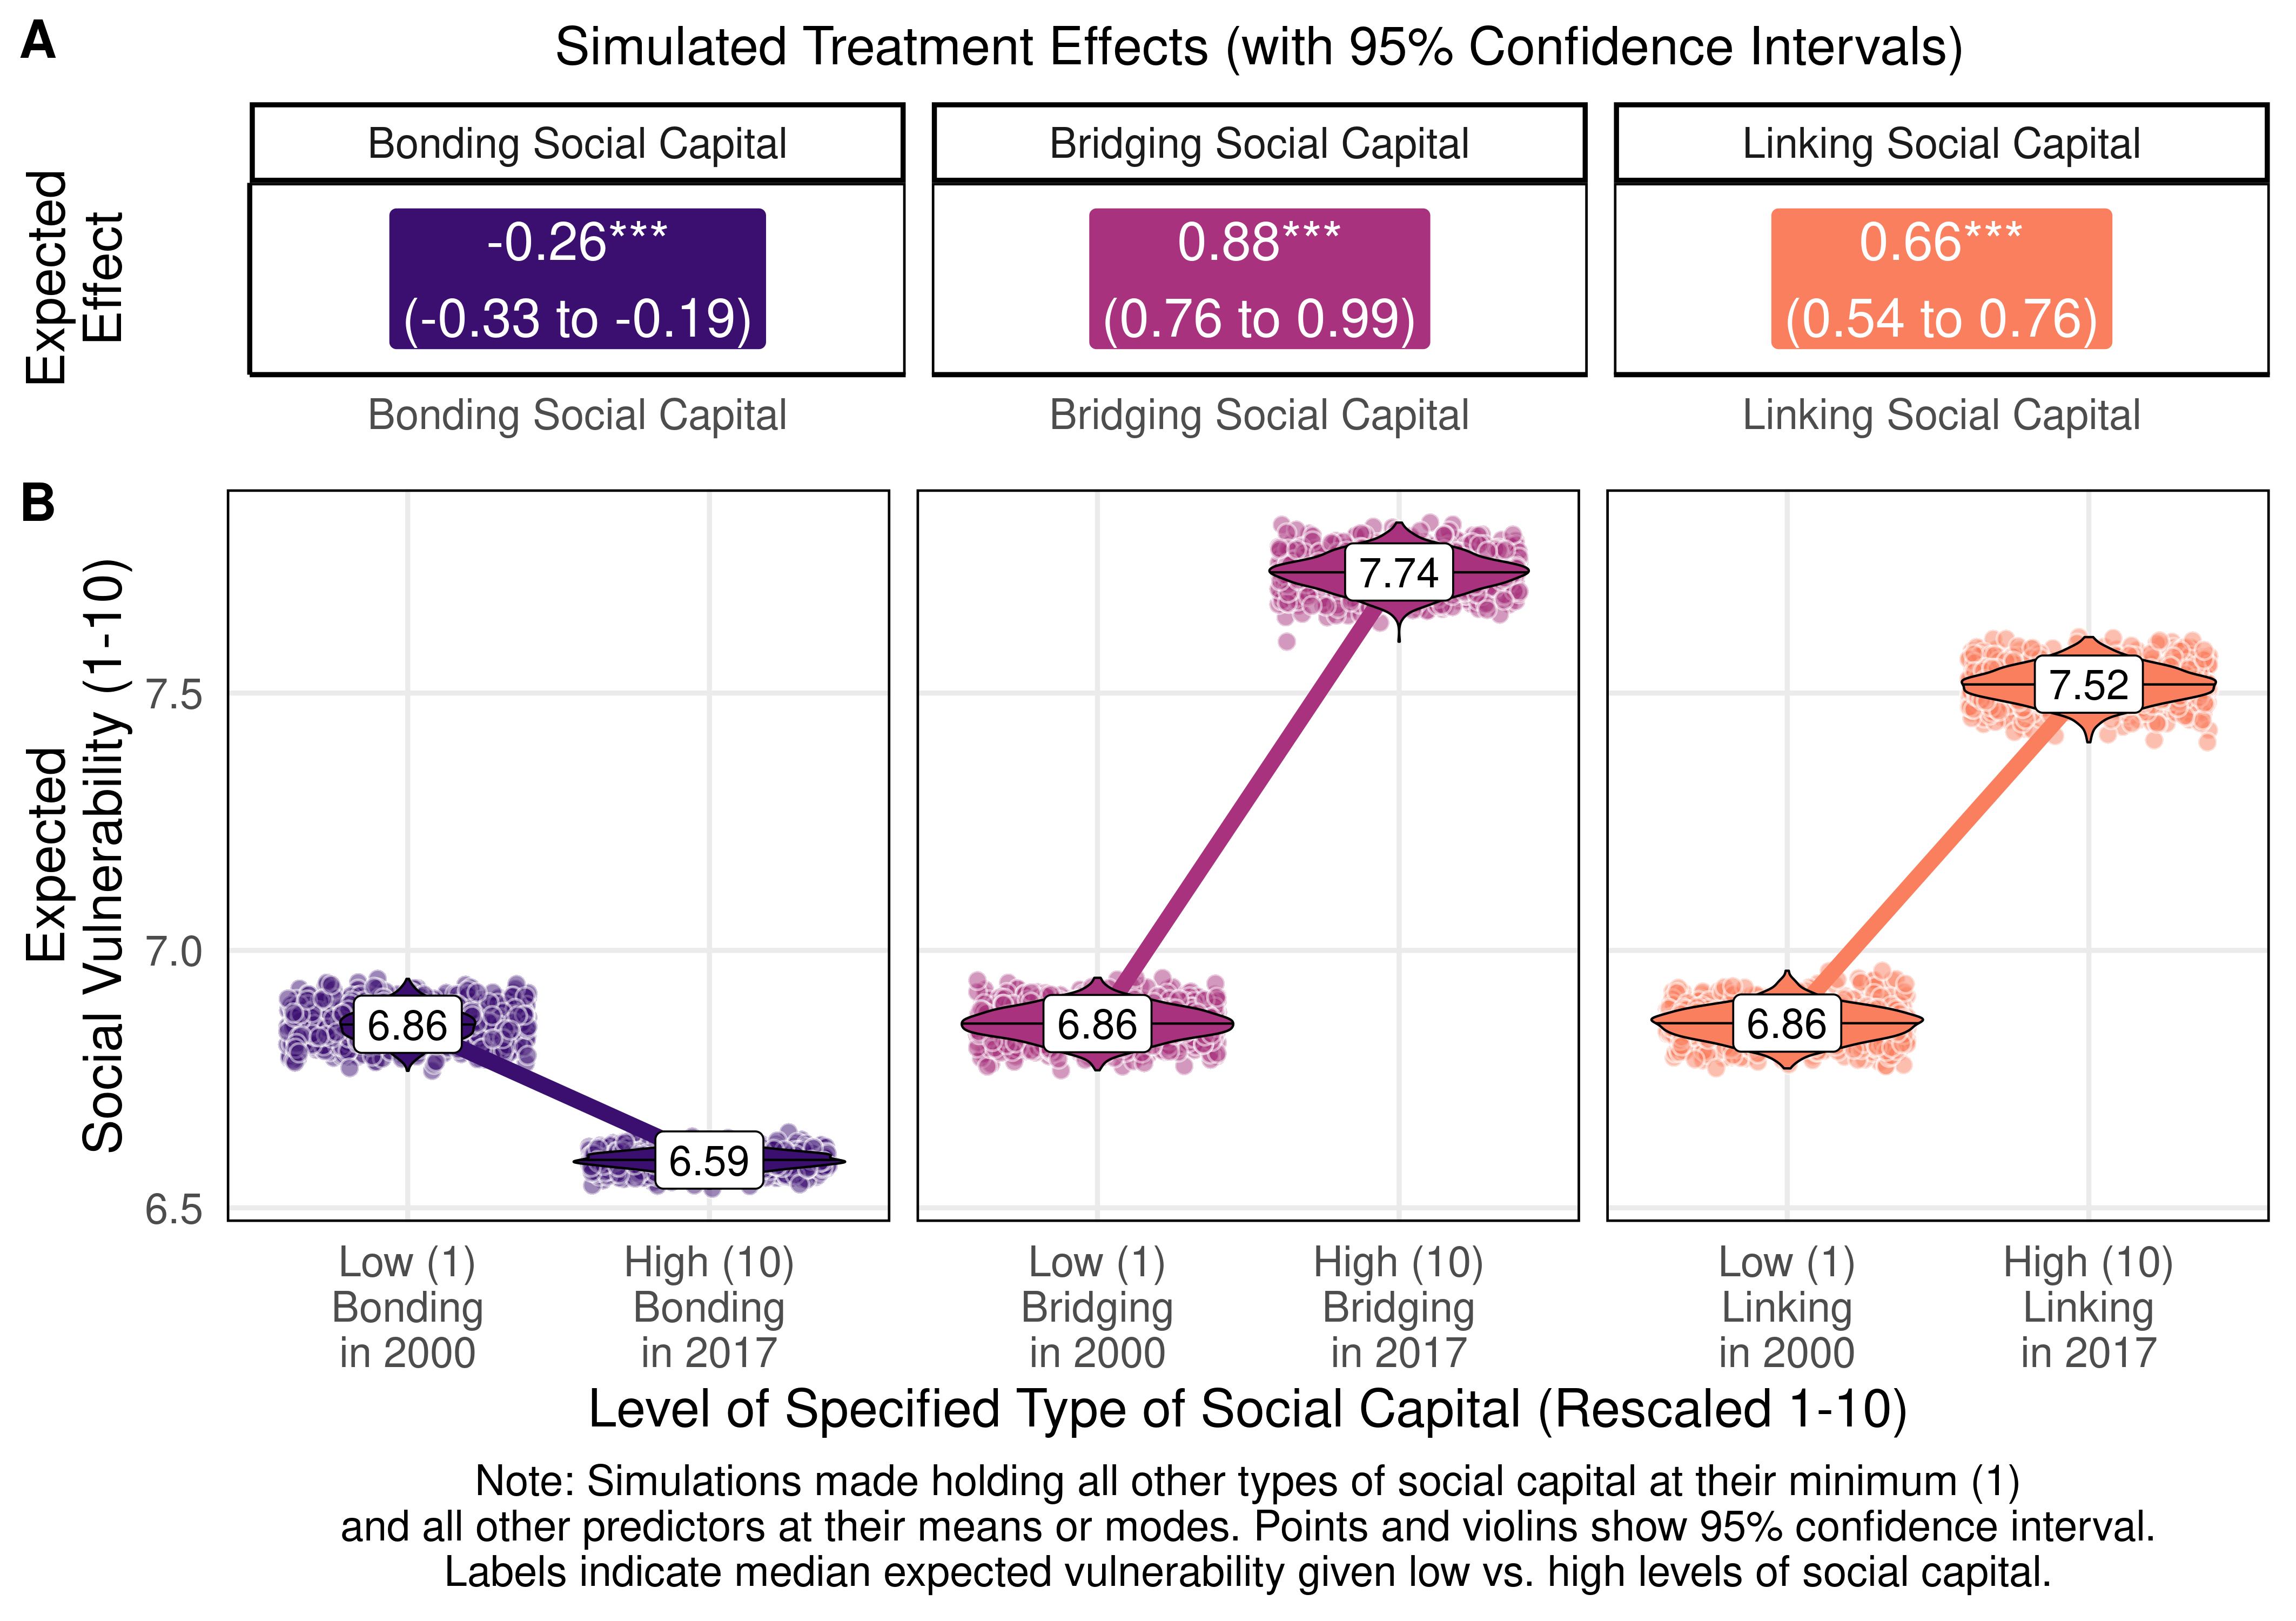
\includegraphics[width=1\linewidth]{did_fd} \caption{Figure 1: Simulated Treatment Effects of Social Capital on Vulnerability (Model 4)}\label{fig:fig1}
\end{figure}
\elandscape
\newpage

\hypertarget{results}{%
\section{Results}\label{results}}

\hypertarget{hypothesis-1-does-bonding-social-capital-decrease-vulnerability}{%
\subsection{Hypothesis 1: Does Bonding Social Capital Decrease
Vulnerability?}\label{hypothesis-1-does-bonding-social-capital-decrease-vulnerability}}

First, we hypothesized that bonding social capital decreases
vulnerability, and we find strong evidence to support this hypothesis.
Our difference-in-differences models found that with each passing year,
cities where bonding social capital increased experienced lower levels
of vulnerability (beta = -0.003, p \textless{} 0.001, Model 4). This
effect was consistent with and without controls (Models 1-4). Our
simulations in \textbf{Figure 1} project that an average city with the
minimum observed level of bonding social capital (1) in 2000 experienced
an expected vulnerability score of 6.86 on a scale from 1-10. But
holding all else equal, an increase in bonding social capital from
minimum (1) in 2000 to maximum levels (10) in 2017 would lead to an
expected decrease in social vulnerability by -0.26 points down to 6.59.
Our fixed effects models (5-8) showed similar outcomes. We found this
when controlling for each type of social capital, annual fixed effects,
and alternative explanations.

\hypertarget{hypothesis-2-does-bridging-social-capital-decrease-vulnerability}{%
\subsection{Hypothesis 2: Does Bridging Social Capital Decrease
Vulnerability?}\label{hypothesis-2-does-bridging-social-capital-decrease-vulnerability}}

Second, we hypothesized that bridging social capital led to decreases in
social vulnerability as well, but this was not the case. Our
difference-in-differences models found a weak positive effect of
bridging social capital for each passing year (beta \textless{} 0.001, p
\textgreater{} 0.10). However, when we simulated the change in expected
vulnerability, our model projected a moderate increase in social
vulnerability of 0.88 (p \textless{} 0.001) if a city with weak social
capital (1) in 2000 developed strong bridging ties (10) by 2017, holding
all else constant.

Our fixed effects models find similarly statistically significant
evidence of a positive effect (beta = 0.023, p \textless{} 0.001). The
positive relationship between bridging capital and vulnerability
increases dramatically once controls are introduced, then decreases
notably (but remains positive) as more controls are added to the model.
This suggests that regional and disaster-related factors influence this
relationship, but it still remains. This indicates that our hypothesis
was incorrect and that bridging ties on their own do not necessarily
reduce vulnerability, but instead are associated with greater
vulnerability.

We expect that bonding social capital decreased vulnerability while
bridging increased vulnerability because these strong bonding ties were
more effective at delivering the aid that residents in vulnerable
communities need; it is not always realistic to assume that weak
bridging ties between members of different social groups with fill gaps
in housing, food, or shelter as well as bonding social ties do.

\hypertarget{hypothesis-3-does-linking-social-capital-decrease-vulnerability}{%
\subsection{Hypothesis 3: Does Linking Social Capital Decrease
Vulnerability?}\label{hypothesis-3-does-linking-social-capital-decrease-vulnerability}}

Third, we hypothesized that linking social capital would limit
vulnerability, but this was also not so. Our difference-in-differences
models found a weak boosting effect (beta = 0.001, p \textless{} 0.001)
given an increase in linking ties each year. Our simulations found the
same, projecting a median expected increase of 0.66 points (p
\textless{} 0.001) in vulnerability from 1 to 10 for city with weak
social ties (1) in 2000 whose linking social capital increased to
maximum levels (10) by 2017. This contrasts with our hypothesis,
indicating that strong linking ties alone will not help residents reduce
vulnerability in their area.

\hypertarget{controls-and-validation}{%
\subsection{Controls and Validation}\label{controls-and-validation}}

Several additional findings indicate added support for our models.
First, in every model included in the difference in differences and
fixed effect models, even as more controls are added, the effects of the
social capital variables on vulnerability remain statistically
significant and the direction of the effect remains consistent.

Second, we saw several other expected associations between vulnerability
and alternative explanations, including governance capacity and city
spending. We found a negative relationship between vulnerability and
each kind of city spending, the strongest of which was with disaster
relief spending. In contrast, we saw a consistent positive relationship
with vulnerability. This matches with what we would expect; governance
capacity and budget alone does not reduce social vulnerability, but city
spending in key priorities could. Coupled with the notable negative
relationships between per-capita disaster spending and vulnerability,
this suggests that the allocation of money toward disaster spending, not
the amount of money that a town has overall, decreases community
vulnerability. In contrast, disaster conditions were linked to greater
vulnerability, which matches with expectations.

Third, the effects of our independent variable variables over time
actually closely match descriptive evidence as well. In Figure 2, we
plotted the changing correlation between vulnerability and each type of
social capital in municipalities for each of 47 prefectures in Japan
(y-axis) over time (x-axis). This allows us to account for both
geography and time. We see that over time, the association between
bonding social capital and vulnerability declined but remained weakly
positive, while the associations between bridging and linking social
capital remained consistent and weak-to-moderately negative.

\newpage
\blandscape

\begin{figure}
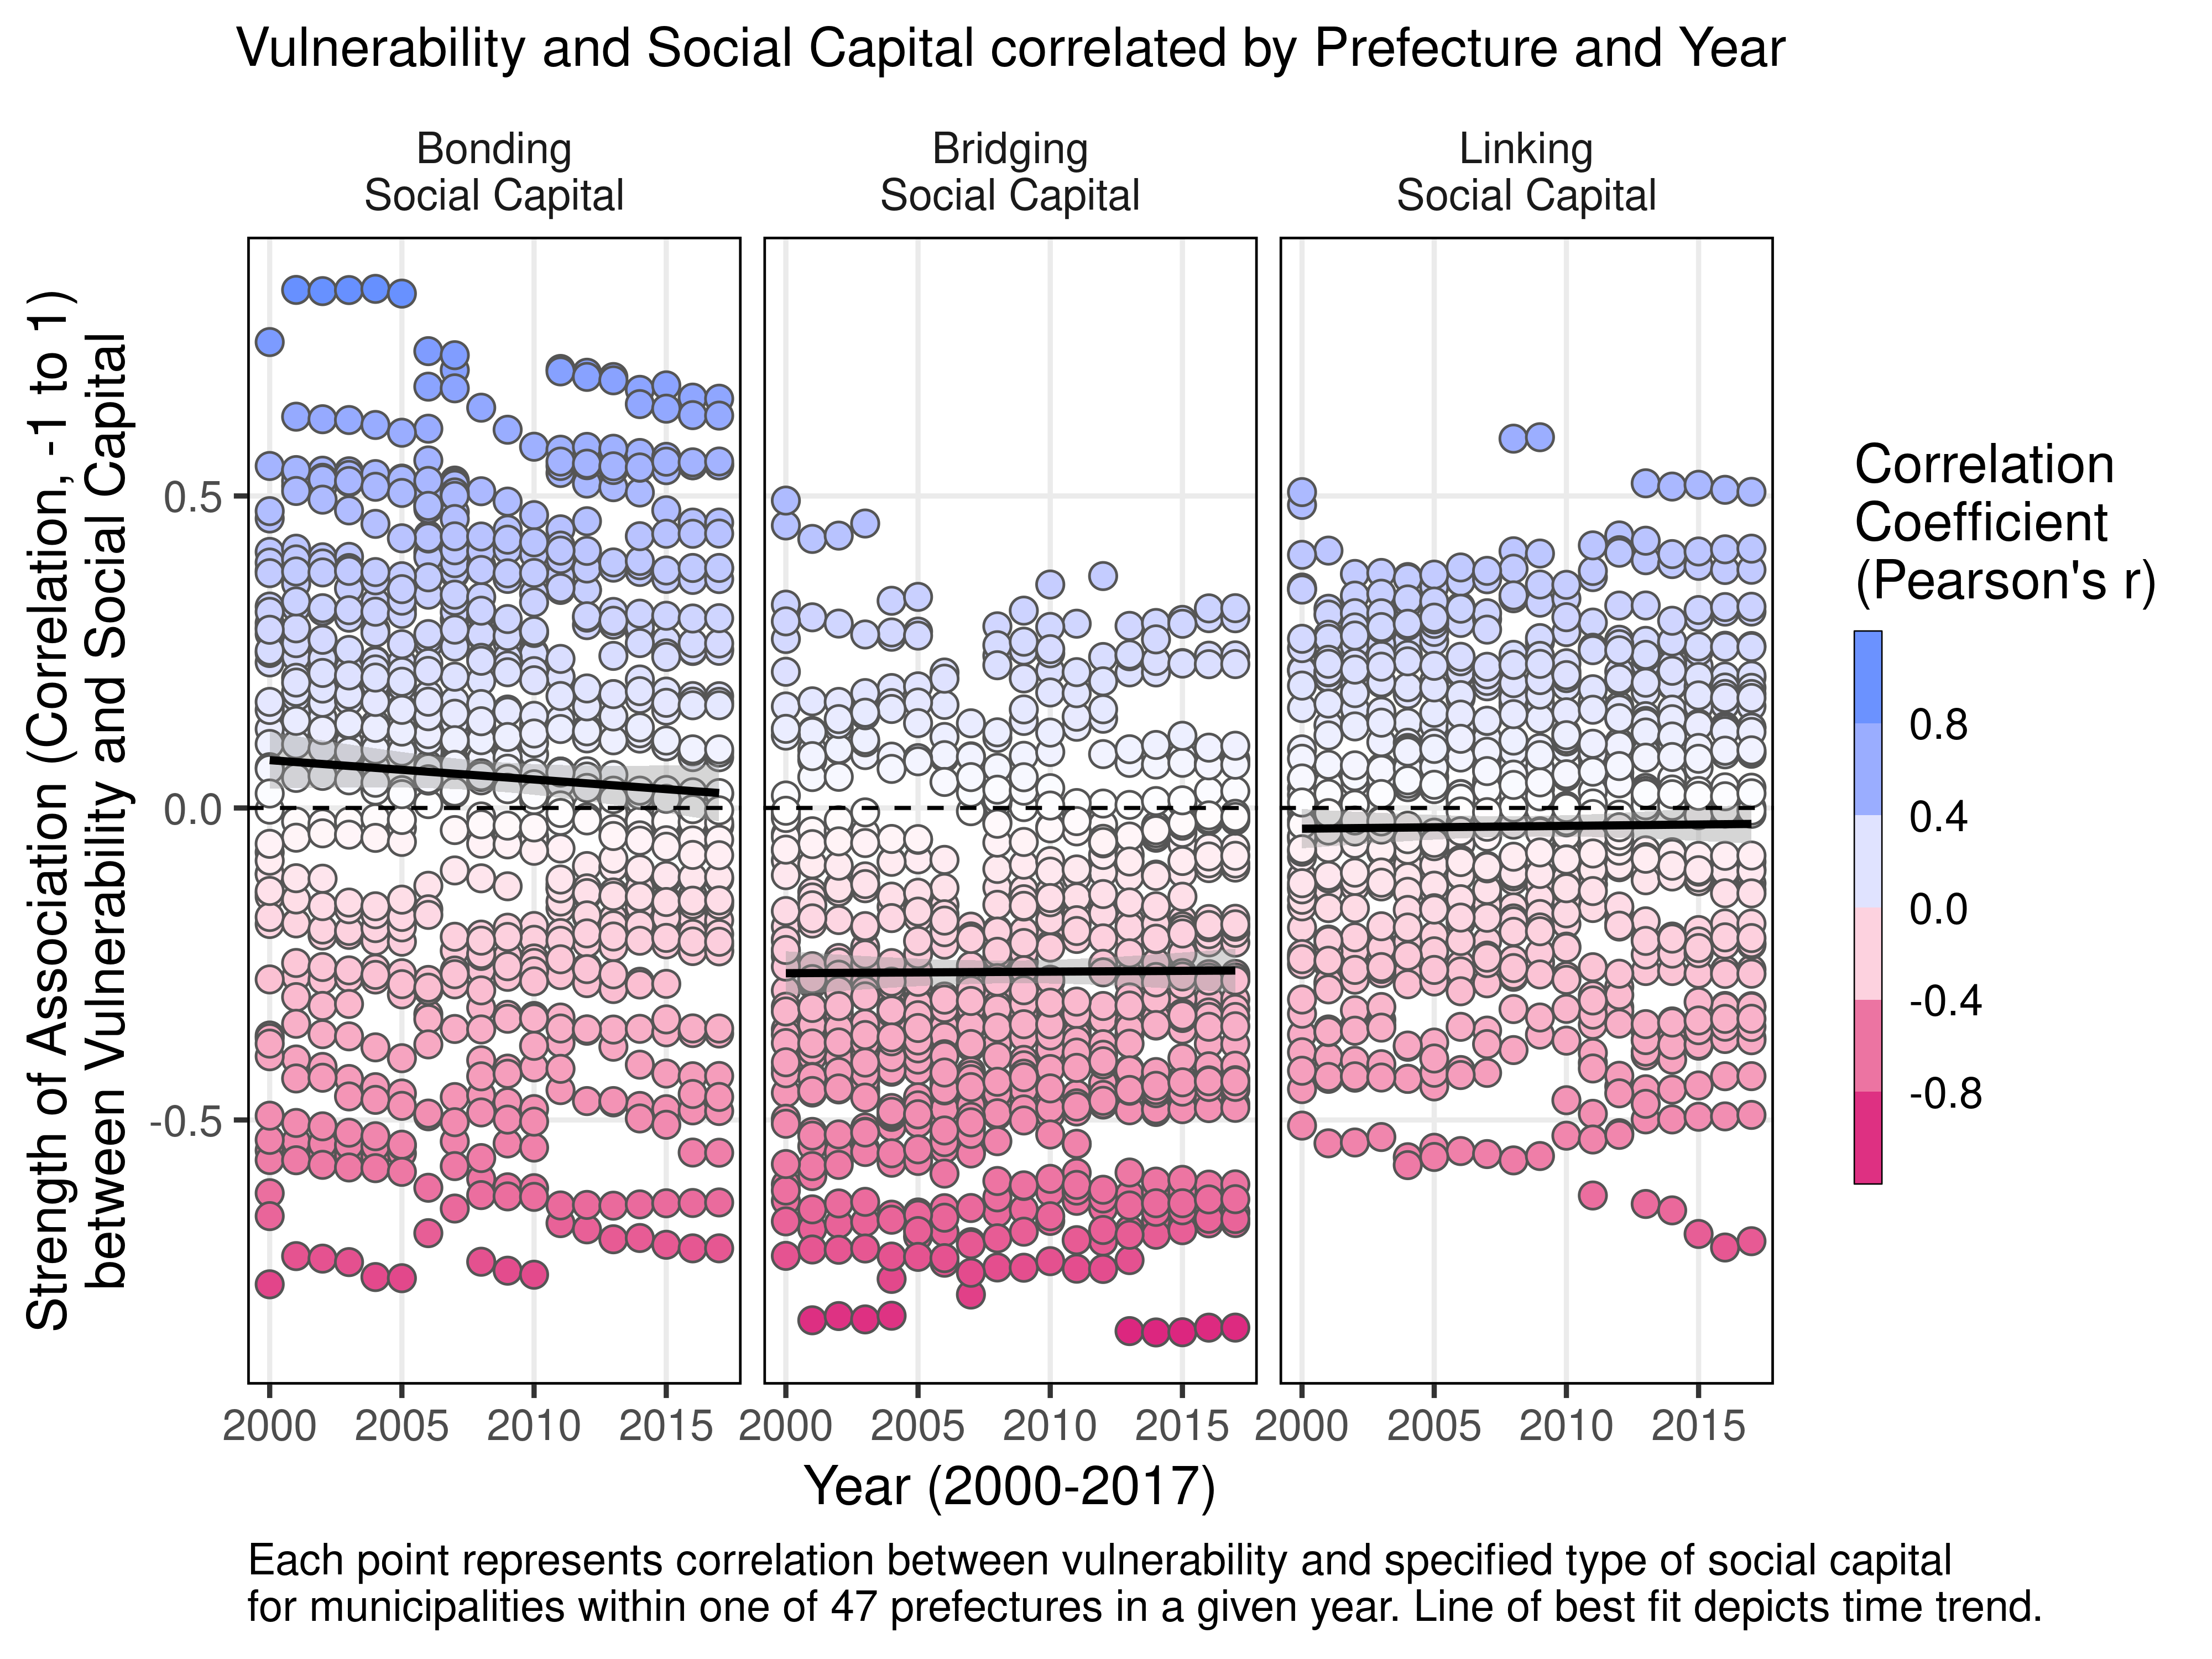
\includegraphics[width=1\linewidth]{fig2_correlation} \caption{Figure 2: Changing Correlations between Social Capital and Vulnerability Over Time}\label{fig:fig2}
\end{figure}

\elandscape
\newpage

\hypertarget{discussion}{%
\section{Discussion}\label{discussion}}

\hypertarget{findings-in-brief}{%
\paragraph{Findings in brief:}\label{findings-in-brief}}

We hypothesized three relationships between social capital and
vulnerability. First, we believed that (\textbf{H1}) stronger bonding
ties would weaken social vulnerability, and that hypothesis is supported
by our research. Second, we believed that (\textbf{H2}) stronger
bridging ties would weaken social vulnerability as well, but our
research suggests that stronger bridging ties actually increase social
vulnerability. Lastly, we hypothesized that (\textbf{H3}) stronger
linking ties would lessen social vulnerability. However, our data shows
a slight positive relationship between linking ties and social
vulnerability, suggesting that stronger linking ties increase
vulnerability.

\hypertarget{value-added}{%
\paragraph{Value Added:}\label{value-added}}

This study is among the first to examine the relationship between social
capital and social vulnerability, especially at a nationwide scale. By
examining the effects of various forms of social relationships on
vulnerability, we can see how interpersonal factors contribute to the
overall resilience of communities. The potential applications for this
kind of analysis are significant. Lawmakers can use this research to
create policies which strengthen and utilize these connections to create
stronger and more resilient communities. Researchers can further analyze
these connections to better understand their relationships with one
another and make more informed suggestions on how communities can be
strengthened through social connections.

The data confirmed our first hypothesis (\textbf{H1}), that increased
bonding ties would decrease vulnerability, but simultaneously
contradicted our second hypothesis (\textbf{H2}), which suggested that
increased bridging ties would likewise decrease vulnerability. This
suggests that in crisis situations, such as in the event of disasters,
reliance on relationships made from bonding ties lessens vulnerability
more than reliance on relationships made from bridging ties. This could
be due to a greater understanding among those with bonding ties of each
other's needs, since they belong to the same in-groups.

Societal norms also often prioritize bonding relationships,
incentivizing people to rely on those relationships or prioritize those
with whom they have these sorts of relationships. The effects of this
are potentially exacerbated by our use of Japan as the case for this
study; strong family and in-group ties are common in Japan (Koyano,
2008), and have been linked to positive health outcomes among vulnerable
individuals in the past (Aida et al., 2017; Aldrich and Kyota, 2017;
Hikichi et al., 2020). Even so, the effects of bonding, in-group social
ties exceeded expectations. This may contribute to the notable negative
relationship between bonding social ties and social vulnerability.

Our data also shows a strong positive relationship between the financial
strength and social vulnerability, while simultaneously showing strong
negative relationships between per-capita spending on disaster
management and social vulnerability. This is an especially important
finding for policy design purposes, since it suggests that it is
increased per-capita expenditures on disaster management, not increased
government capacity (financial strength), that reduces social
vulnerability. That is, the amount of money spent per-person on disaster
management is far more important and effective than the amount of money
that a city has overall. This means that wealthier cities tend to see
greater levels of social vulnerability, after accounting for other
controls. Read positively, this suggests that, richer or poorer, any
city can better protect its citizens by investing in disaster
management. We interpret associations for control variables cautiously,
since this quasi-experiment is designed to test effects of social
capital, using governance capacity and spending as just controls.
However, we encourage future studies to implement quasi- or natural
experiments to test these associations in greater detail.

\hypertarget{limitations}{%
\paragraph{Limitations:}\label{limitations}}

This study comes with several limitations. First, we extrapolated
results from years of Japanese census data, therefore making our
quasi-experiments `observational.' Considering this less-controlled
environment, we relied upon statistical controls to adjust for
population, governance capacity, policy tool choice, disaster damage,
migration impacts on social cohesion, temporal variation, and regional
differences.

Second, we did not control for socioeconomic status, gender, or other
vulnerability-related measures to avoid endogeneity bias, because these
indicators are already integrated into the outcome variable itself.

Third, our final models do not include measures for social assistance
since they were already included in our vulnerability measures. Though
this was done to prevent collinearity, it also meant that we could not
investigate the relationship between social assistance and vulnerability
through our final models. (Still, our findings persisted even when we
controlled for spending on social assistance.) This is an exciting area
for future research, and we encourage future scholars to examine
relationships between social welfare support and each aspect of
vulnerability independently.

Fourth, this study examined a single country, Japan, and this raises
questions about in what contexts these results are generalizable. Given
that Japan's 1741 municipalities are highly susceptible to typhoons,
earthquakes, and tsunami most of every year, the authors hope that our
findings on the correlates of vulnerability present value added, even in
isolation. Fortunately, however, Japan is not a unique case, but rather
the 3rd largest economy in the world, and a major industrialized
democracy. We anticipate that friendship, family, and ties to colleagues
and acquaintances also play close roles in supporting and alleviating
vulnerability in other industrialized democracies like the US, Germany,
Taiwan, South Korea, and many other states. We encourage future
comparative research, such as efforts using the Global Social Survey, to
investigate these questions.

\hypertarget{policy-implications}{%
\paragraph{Policy Implications}\label{policy-implications}}

Finally, this research comes with several implications for policymakers.

\begin{itemize}
\item
  This study's findings suggest cities may benefit from leveraging
  existing bonding social ties to reduce social vulnerability in cities,
  drawing from an array of inexpensive programs and policy tools to
  promote bonding ties, by bringing families, friends, and neighbors
  together. Unfortunately, this differs from recovery approaches to the
  2011 tsunami, where municipalities primarily rebuilt according to
  central government-issued plans that emphasized infrastructural
  solutions like seawalls, leaving out community-cohesion building
  efforts and limiting community participation (Cheek, 2020).
\item
  Since these people may already share traits in common, events which
  create ties among these people can be advertised as designated spaces
  for these people to congregate, share their experiences, and make
  friends. Examples of such events include cultural group meetings,
  social events for senior citizens, and religious holiday celebrations.
  These events seek to reinforce trust and mutual support among these
  social circles.
\item
  Such groups need \emph{places to gather and invest their time,
  frequently.} This echoes recent calls for greater investment in
  cities' `social infrastructure', referring to the community centers,
  places of worship, social businesses, and parks that bring people
  together to form social ties (Fraser et al., 2021b; Klinenberg, 2018).
\item
  Examples of institutional methods for strengthening in-group ties
  include weekly religious services organized by places of worship,
  community classes organized by schools, and activities for elders and
  family members organized by community centers or retirement homes
  (Aldrich and Kyota, 2017). Japan already has invested in a robust
  system of community centers to support the social wellbeing and health
  of elders, although some are more accessible and active than others
  (Ghezelloo et al., 2022). With only slight adjustments, these centers
  could help reach vulnerable non-elders as well.
\end{itemize}

\hypertarget{directions-for-further-research}{%
\paragraph{Directions for Further
Research}\label{directions-for-further-research}}

Social capital and social vulnerability have great potential
applications in development studies (Woolcock and Narayan, 2000);
development inequities still loom large, with low income countries
suffering disproportionately high rates of fatalities from disasters
(Mochizuki et al., 2014). Neoliberal development theory prioritized
development ideas and policy from Global North states, often to the
detriment of Global South states (Stiglitz, 2002). In contrast, social
capital perspectives place greater attention on what local residents can
achieve, highlighting grassroots-level mutual aid and organizing that
spurs community resilience in vulnerable communities during
reconstruction (Monteil et al., 2020). Past studies conceptualized
social capital-related concepts as ``open'' and ``limited access''
orders (North and Weingast, 2009), describing how effectively citizens
and leverage their relationships with authorities to access to political
and economic support; others described the same concept as local
officials' degree of ``embeddedness'' in community organizations (Tsai,
2007). Both concepts are near equivalents of linking capital. There is
ripe opportunity for testing how other types of social relationships
affect state development.

Though our study finds a consistent negative effect of bonding capital
on vulnerability, the jury remains out on the effects of other types of
social capital on social vulnerability; the literature strongly suggests
that bridging ties benefit vulnerable groups during and after crisis
(Aldrich and Sawada, 2015; Cox and Perry, 2011; Elliott et al., 2010;
Fraser et al., 2021a); although weak bridging ties might not be enough
to change the financial security of a household, we suspect that
simultaneous investments in bonding and bridging ties might be
beneficial in communities. We encourage future studies, field
experiments, and more to investigate these important questions.

Further, though we found that bonding social capital was linked to
\textbf{\emph{lower}} social vulnerability, literature suggests that
this is only true to an extent. In-group ties can also form,
regrettably, among extremist and supremacist groups. We would expect
that strong bonding ties within these groups are detrimental to social
vulnerability in the short and long term, since such groups may become
motivated to discriminate or commit acts of violence against those
outside of their group (Alcorta et al., 2020; Aldrich and Crook, 2008;
Aldrich et al., 2018). Further research could be done to discover the
threshold at which bonding social capital becomes detrimental, rather
than beneficial, to the goal of decreasing social vulnerability.

By examining the nuances of bonding in-group social ties in
vulnerability, we hope this research will lead to renewed investigations
of the potentials for social capital-based interventions to reduce
vulnerability and improve cities' sustainable development overall.

\hypertarget{credit-author-statement}{%
\section{CRediT author statement}\label{credit-author-statement}}

Timothy Fraser: writing - original draft; formal analysis; methodology;
visualization; conceptualization; supervision. Nicole Naquin: writing -
original draft; formal analysis; visualization.

\hypertarget{declaration-of-interests}{%
\section{Declaration of interests}\label{declaration-of-interests}}

The authors declare that they have no known competing financial
interests or personal relationships that could have appeared to
influence the work reported in this paper.

\hypertarget{data-availability}{%
\section{Data Availability}\label{data-availability}}

All data and replication code for this study is publicly available on
the Harvard Dataverse at: \url{https://doi.org/10.7910/DVN/YCUNHJ}

\singlespacing

\hypertarget{references}{%
\section*{References}\label{references}}
\addcontentsline{toc}{section}{References}

\hypertarget{refs}{}
\begin{CSLReferences}{1}{0}
\leavevmode\vadjust pre{\hypertarget{ref-abadie_et_al_2015}{}}%
Abadie, A., Diamond, A., Hainmueller, J., 2015. Comparative politics and
the synthetic control method. American Journal of Political Science 59,
495--510.
doi:\href{https://doi.org/10.1111/ajps.12116}{10.1111/ajps.12116}

\leavevmode\vadjust pre{\hypertarget{ref-abadie_et_al_2010}{}}%
Abadie, A., Diamond, D., Hainmueller, J., 2010. Synthetic control
methods for comparative case studies: Estimating the effect of
california's tobacco control program. Journal of the American
Statistical Association 105, 493--505.
doi:\href{https://doi.org/10.1198/jasa.2009.ap08746}{10.1198/jasa.2009.ap08746}

\leavevmode\vadjust pre{\hypertarget{ref-adalja_et_al_2014}{}}%
Adalja, A.A., Watson, M., Bouri, N., Minton, K., Morhard, R.C., Toner,
E.S., 2014. Absorbing citywide patient surge during hurricane sandy: A
case study in accommodating multiple hospital evacuations. Annals of
emergency medicine 64, 66--73.

\leavevmode\vadjust pre{\hypertarget{ref-aida_et_al_2017}{}}%
Aida, J., Hikichi, H., Matsuyama, Y., Sato, Y., Tsuboya, T., Tabuchi,
T., Koyama, S., Subramanian, S.V., Kondo, K., Osaka, K., Kawachi, I.,
2017. Risk of mortality during and after the 2011 great east JApan
earthquake and tsunami among older coastal residents. Scientific Reports
7, 16591.

\leavevmode\vadjust pre{\hypertarget{ref-alcorta_et_al_2020}{}}%
Alcorta, L., Smits, J., Swedlund, H.J., Jong, E. de, 2020. The 'dark
side' of social capital: A cross-national examination of the
relationship between social capital and violence in africa. Social
Indicators Research 149, 445--465.

\leavevmode\vadjust pre{\hypertarget{ref-aldrich_and_crook_2008}{}}%
Aldrich, Daniel P., Crook, K., 2008. Strong civil society as a
double-edged sword: Siting trailers in post-katrina new orleans.
Political Research Quarterly 61, 379--389.

\leavevmode\vadjust pre{\hypertarget{ref-aldrich_2011}{}}%
Aldrich, D.P., 2011. The power of people: Social capital's role in
recovery from the 1995 kobe earthquake. Natural hazards 56, 595--611.

\leavevmode\vadjust pre{\hypertarget{ref-aldrich_2012}{}}%
Aldrich, D.P., 2012. Building resilience: Social capital in
post-disaster recovery. University of Chicago Press, Chicago, IL.

\leavevmode\vadjust pre{\hypertarget{ref-aldrich_2019}{}}%
Aldrich, D.P., 2019. Black wave: How networks and governance shaped
japan's 3/11 disasters. University of Chicago Press, Chicago, IL.

\leavevmode\vadjust pre{\hypertarget{ref-aldrich_and_kiyota_2017}{}}%
Aldrich, D.P., Kyota, E., 2017. Creating community resilience through
elder-led physical and social infrastructure. Disaster medicine and
public health preparedness 11, 120--126.

\leavevmode\vadjust pre{\hypertarget{ref-aldrich_and_meyer_2015}{}}%
Aldrich, D.P., Meyer, M.A., 2015. Social capital and community
resilience. American Behavioral Scientist 59, 254--269.
doi:\href{https://doi.org/10.1177/0002764214550299}{10.1177/0002764214550299}

\leavevmode\vadjust pre{\hypertarget{ref-aldrich_et_al_2018}{}}%
Aldrich, D.P., Page-Tan, C., Fraser, T., 2018.
\href{https://beta.irgc.org/wp-content/uploads/2018/12/Aldrich-et-al-for-IRGC-Resilience-Guide-Vol-2-2018.pdf}{A
janus-faced resource: Social capital and resilience trade-offs.}, in:
Trump, B.D. (Ed.),. EPFL International Risk Governance Center, Lausanne,
CH.

\leavevmode\vadjust pre{\hypertarget{ref-aldrich_and_sawada_2015}{}}%
Aldrich, D.P., Sawada, Y., 2015. The physical and social determinants of
mortality in the 3.11 tsunami. Social Science \& Medicine 124, 66--75.
doi:\href{https://doi.org/10.1016/j.socscimed.2014.11.025}{10.1016/j.socscimed.2014.11.025}

\leavevmode\vadjust pre{\hypertarget{ref-alesina_et_al_1999}{}}%
Alesina, A., Baqir, R., Easterly, W., 1999. {Public Goods and Ethnic
Divisions}. The Quarterly Journal of Economics 114, 1243--1284.
doi:\href{https://doi.org/10.1162/003355399556269}{10.1162/003355399556269}

\leavevmode\vadjust pre{\hypertarget{ref-ando_2015}{}}%
Ando, M., 2015. Dreams of urbanization: Quantitative case studies on the
local impacts of nuclear power facilities using the synthetic control
method. Journal of Urban Economics 85, 68--85.
doi:\url{https://doi.org/10.1016/j.jue.2014.10.005}

\leavevmode\vadjust pre{\hypertarget{ref-angrist_and_pischke_2008}{}}%
Angrist, J.D., Pischke, J.-S., 2008. Mostly harmless econometrics: An
empiricist's companion. Princeton University Press, Princeton, New
Jersey.

\leavevmode\vadjust pre{\hypertarget{ref-bollyky_et_al_2019}{}}%
Bollyky, T.J., Templin, T., Cohen, M., Schoder, D., Dieleman, J.L.,
Wigley, S., 2019. The relationships between democratic experience, adult
health, and cause-specific mortality in 170 countries between 1980 and
2016: An observational analysis. The Lancet 393, 1628--1640.

\leavevmode\vadjust pre{\hypertarget{ref-burke_and_stephens_2017}{}}%
Burke, M.J., Stephens, J.C., 2017. Energy democracy: Goals and policy
instruments for sociotechnical transitions. Energy research \& social
science 33, 35--48.

\leavevmode\vadjust pre{\hypertarget{ref-campbell_1996}{}}%
Campbell, S., 1996. Green cities, growing cities, just cities?: Urban
planning and the contradictions of sustainable development. Journal of
the American Planning Association 62, 296--312.

\leavevmode\vadjust pre{\hypertarget{ref-catalinac_et_al_2020}{}}%
Catalinac, A., Mesquita, B.B. de, Smith, A., 2020. A tournament theory
of pork barrel politics: The case of japan. Comparative Political
Studies 53, 1619--1655.
doi:\href{https://doi.org/10.1177/0010414019897677}{10.1177/0010414019897677}

\leavevmode\vadjust pre{\hypertarget{ref-chapman_et_al_2016}{}}%
Chapman, A.J., McLellan, B., Tezuka, T., 2016. Proposing an evaluation
framework for energy policy making incorporating equity: Applications in
australia. Energy Research \& Social Science 21, 54--69.

\leavevmode\vadjust pre{\hypertarget{ref-chapman_and_shigetomi_2018}{}}%
Chapman, A., Shigetomi, Y., 2018. Visualizing the shape of society: An
analysis of public bads and burden allocation due to household
consumption using an input-output approach. Science of The Total
Environment 639, 385--396.

\leavevmode\vadjust pre{\hypertarget{ref-cheek_2020}{}}%
Cheek, W., 2020. \href{https://doi.org/10.1108/DPM-12-2019-0374}{The
paradox of community involvement: Rebuilding minamisanriku}. Disaster
Prevention and Management 29, 893--907.

\leavevmode\vadjust pre{\hypertarget{ref-choi_et_al_2018}{}}%
Choi, Y., Kwon, Y.-H., Kim, J., 2018. The effect of the social networks
of the elderly on housing choice in korea. Habitat International 74,
1--8.

\leavevmode\vadjust pre{\hypertarget{ref-collins_et_al_2021}{}}%
Collins, J., Polen, A., McSweeney, K., Colón-Burgos, D., Jernigan, I.,
2021. Hurricane risk perceptions and evacuation decision-making in the
age of COVID-19. Bulletin of the American Meteorological Society 102,
E836--E848.

\leavevmode\vadjust pre{\hypertarget{ref-cox_et_al_2011}{}}%
Cox, Robin S., Perry, K.-M.E., 2011. Like a fish out of water:
Reconsidering disaster recovery and the role of place and social capital
in community disaster resilience. American Journal of Community
Psychology 395--411.

\leavevmode\vadjust pre{\hypertarget{ref-craig_2019}{}}%
Craig, R.K., 2019.
\href{https://doi.org/10.1007/s10584-018-2203-5}{Coastal adaptation,
government-subsidized insurance, and perverse incentives to stay}.
Climatic Change 152, 215--226.

\leavevmode\vadjust pre{\hypertarget{ref-cutter_et_al_2003}{}}%
Cutter, S.L., Boruff, B.J., Shirley, L.W., 2003. Social vulnerability to
environmental hazards. Social Science Quarterly 84, 242--261.
doi:\href{https://doi.org/10.1111/1540-6237.8402002}{10.1111/1540-6237.8402002}

\leavevmode\vadjust pre{\hypertarget{ref-cutter_and_emrich_2006}{}}%
Cutter, S.L., Emrich, C.T., 2006. Moral hazard, social catastrophe: The
changing face of vulnerability along the hurricane coasts. Annals of the
American Academy of Political and Social Science 604, 102--112.

\leavevmode\vadjust pre{\hypertarget{ref-cutter_et_al_2006}{}}%
Cutter, S.L., Emrich, C.T., Mitchell, J.T., Boruff, B.J., Gall, M.,
Schmidtlein, M.C., Burton, C.G., Melton, G., 2006. The long road home:
Race, class, and recovery from hurricane katrina. Environment: Science
and Policy for Sustainable Development 48, 8--20.

\leavevmode\vadjust pre{\hypertarget{ref-cutter_and_finch_2008}{}}%
Cutter, S.L., Finch, C., 2008. Temporal and spatial changes in social
vulnerability to natural hazards. Proceedings of the national academy of
sciences 105, 2301--2306.

\leavevmode\vadjust pre{\hypertarget{ref-daoud_et_al_2016}{}}%
Daoud, A., Halleröd, B., Guha-Sapir, D., 2016. What is the association
between absolute child poverty, poor governance, and natural disasters?
A global comparison of some of the realities of climate change. PLoS one
11, e0153296.

\leavevmode\vadjust pre{\hypertarget{ref-das_2019}{}}%
Das, S., 2019. Evaluating climate change adaptation through evacuation
decisions: A case study of cyclone management in india. Climatic Change
152, 291--305.

\leavevmode\vadjust pre{\hypertarget{ref-deng_et_al_2021}{}}%
Deng, H., Aldrich, D.P., Danziger, M.M., Gao, J., Phillips, N.E.,
Cornelius, S.P., Wang, Q.R., 2021.
\href{https://doi.org/10.1057/s41599-021-00824-8}{High-resolution human
mobility data reveal race and wealth disparities in disaster evacuation
patterns}. Humanities and Social Sciences Communications 8, 144.

\leavevmode\vadjust pre{\hypertarget{ref-deyoung_et_al_2016}{}}%
DeYoung, S.E., Wachtendorf, T., Davidson, R.A., Xu, K., Nozick, L.,
Farmer, A.K., Zelewicz, L., 2016. A mixed method study of hurricane
evacuation: Demographic predictors for stated compliance to voluntary
and mandatory orders. Environmental hazards 15, 95--112.
doi:\href{https://doi.org/10.1080/17477891.2016.1140630}{10.1080/17477891.2016.1140630}

\leavevmode\vadjust pre{\hypertarget{ref-domingue_and_emrich_2019}{}}%
Domingue, S.J., Emrich, C.T., 2019. Social vulnerability and procedural
equity: Exploring the distribution of disaster aid across counties in
the united states. American review of public administration 49,
897--913.
doi:\href{https://doi.org/10.1177/0275074019856122}{10.1177/0275074019856122}

\leavevmode\vadjust pre{\hypertarget{ref-drakes_et_al_2021}{}}%
Drakes, Oronde, Tate, Eric, Rainey, Jayton, Brody, S., 2021.
\href{https://doi.org/10.1016/j.ijdrr.2020.102010}{Social vulnerability
and short-term disaster assistance in the united states}. International
Journal of Disaster Risk Reduction 53, 102010.

\leavevmode\vadjust pre{\hypertarget{ref-edgington_2010}{}}%
Edgington, D.W., 2010. Reconstructing kobe: The geography of crisis and
opportunity. University of British Columbia Press, Vancouver.

\leavevmode\vadjust pre{\hypertarget{ref-elliott_et_al_2010}{}}%
Elliott, J.R., Haney, T.J., Sams-Abiodun, P., 2010. Limits to social
capital: Comparing network assistance in two new orleans neighborhoods
devastated by hurricane katrina. The Sociological Quarterly 51,
624--648.
doi:\href{https://doi.org/10.1111/j.1533-8525.2010.01186.x}{10.1111/j.1533-8525.2010.01186.x}

\leavevmode\vadjust pre{\hypertarget{ref-emrich_et_al_2020}{}}%
Emrich, Christopher T., Tate, Eric, Larson, Sarah E., Zhou, Y., 2020.
Measuring social equity in flood recovery funding. Environmental Hazards
19, 228--250.
doi:\href{https://doi.org/10.1080/17477891.2019.1675578}{10.1080/17477891.2019.1675578}

\leavevmode\vadjust pre{\hypertarget{ref-enarson_1998}{}}%
Enarson, E., 1998. Through women's eyes: A gendered research agenda for
disaster social science. Disasters 22, 157--173.

\leavevmode\vadjust pre{\hypertarget{ref-farag_et_al_2013}{}}%
Farag, N.H., Rey, A., Noe, R., Bayleyegn, T., Wood, A.D., Zane, D.,
2013. Evaluation of the american red cross disaster-related mortality
surveillance system using hurricane ike data---texas 2008. Disaster
medicine and public health preparedness 7, 13--19.

\leavevmode\vadjust pre{\hypertarget{ref-finch_et_al_2010}{}}%
Finch, C., Emrich, Christopher.T., Cutter, S.L., 2010. Disaster
disparities and differential recovery in new orleans. Population and
Environment 31, 179--202.

\leavevmode\vadjust pre{\hypertarget{ref-flanagan_et_al_2011}{}}%
Flanagan, B.E., Gregory, E.W., Hallisey, E.J., Heitgerd, J.L., Lewis,
B., 2011. A social vulnerability index for disaster management. Journal
of homeland security and emergency management 8.

\leavevmode\vadjust pre{\hypertarget{ref-flanagan_et_al_2018}{}}%
Flanagan, B.E., Hallisey, E.J., Adams, E., Lavery, A., 2018. Measuring
community vulnerability to natural and anthropogenic hazards: The
centers for disease control and prevention's social vulnerability index.
Journal of environmental health 80, 34.

\leavevmode\vadjust pre{\hypertarget{ref-fothergill_et_al_1999}{}}%
Fothergill, A., Maestas, E.G., Darlington, J.D., 1999. Race, ethnicity
and disasters in the united states: A review of the literature.
Disasters 23, 156--173.

\leavevmode\vadjust pre{\hypertarget{ref-fothergill_and_peek_2004}{}}%
Fothergill, A., Peek, L.A., 2004. Poverty and disasters in the united
states: A review of recent sociological findings. Natural Hazards 32,
89--110.

\leavevmode\vadjust pre{\hypertarget{ref-fraser_2021_IJDRR}{}}%
Fraser, T., 2021.
\href{https://doi.org/10.1016/j.ijdrr.2020.101965}{Japanese social
capital and social vulnerability indices: Measuring drivers of community
resilience 2000-2017}. International Journal of Disaster Risk Reduction
52, 1--11.

\leavevmode\vadjust pre{\hypertarget{ref-fraser_and_aldrich_2021_SR}{}}%
Fraser, T., Aldrich, D.P., 2021.
\href{https://doi.org/10.1038/s41598-021-81001-4}{The dual effect of
social ties on COVID-19 spread in japan}. Scientific Reports 11, 1--12.

\leavevmode\vadjust pre{\hypertarget{ref-fraser_et_al_2021_GEC}{}}%
Fraser, T., Aldrich, D.P., Small, A., 2021b. Seawalls or social
recovery? The role of policy networks and design in disaster recovery.
Global environmental change 70, 102342.
doi:\href{https://doi.org/10.1016/j.gloenvcha.2021.102342}{10.1016/j.gloenvcha.2021.102342}

\leavevmode\vadjust pre{\hypertarget{ref-fraser_et_al_2021_NH}{}}%
Fraser, T., Aldrich, D.P., Small, A., 2021a. Connecting social capital
and vulnerability: Citation network analysis of disaster studies.
Natural hazards review 22.
doi:\href{https://doi.org/10.1061/(ASCE)NH.1527-6996.0000469}{10.1061/(ASCE)NH.1527-6996.0000469}

\leavevmode\vadjust pre{\hypertarget{ref-fraser_et_al_2022_EIST}{}}%
Fraser, T., Bancroft, M., Small, A., Cunningham, L., 2022. Leaders or
networkers? The role of mayors in renewable energy transition.
Environmental Innovation and Societal Transitions 42, 301--316.
doi:\url{https://doi.org/10.1016/j.eist.2022.01.003}

\leavevmode\vadjust pre{\hypertarget{ref-fraser_et_al_2021_CRM}{}}%
Fraser, T., Morikawa, L., Aldrich, D.P., 2021c. Rumor has it: The role
of social ties and misinformation in evacuation to nearby shelters after
disaster. Climate Risk Management 33, 100320.

\leavevmode\vadjust pre{\hypertarget{ref-fraser_and_temocin_2021_CC}{}}%
Fraser, T., Temocin, P., 2021. Grassroots vs. Greenhouse: The role of
environmental organizations in reducing carbon emissions. Climatic
Change 169, 1--21.

\leavevmode\vadjust pre{\hypertarget{ref-fukui_and_fukai_1996}{}}%
Fukui, H., Fukai, S.N., 1996. Pork barrel politics, networks, and local
economic development in contemporary japan. Asian Survey 36, 268--286.
doi:\href{https://doi.org/10.2307/2645692}{10.2307/2645692}

\leavevmode\vadjust pre{\hypertarget{ref-ghezelloo_et_al_2022}{}}%
Ghezelloo, Y., Hokugo, A., Maly, Elizabeth, Shiomi, Y., 2022.
Authorization and levels of justice in recovery of gathering spaces
after the great east japan earthquake and tsunami 2011. Progress in
Disaster Science 13, 100217.

\leavevmode\vadjust pre{\hypertarget{ref-goldsmith_et_al_2022}{}}%
Goldsmith, L., Raditz, V., Méndez, M., 2022.
\href{https://doi.org/10.1111/disa.12509}{Queer and present danger:
Understanding the disparate impacts of disasters on LGBTQ+ communities}.
Disasters.

\leavevmode\vadjust pre{\hypertarget{ref-griego_et_al_2020}{}}%
Griego, Angel L., Flores, Aaron B., Collins, Timothy W., Grineski, S.E.,
2020. \href{https://doi.org/10.1016/j.ijdrr.2020.101766}{Social
vulnerability, disaster assistance, and recovery: A population-based
study of hurricane harvey in greater houston, texas}. International
Journal of Disaster Risk Reduction 51, 101766.

\leavevmode\vadjust pre{\hypertarget{ref-haddad_2007}{}}%
Haddad, M.A., 2007. Transformation of japan's civil society landscape.
Journal of East Asian Studies 7, 413--437.

\leavevmode\vadjust pre{\hypertarget{ref-hallerod_et_al_2013}{}}%
Halleröd, B., Rothstein, B., Daoud, A., Nandy, S., 2013. Bad governance
and poor children: A comparative analysis of government efficiency and
severe child deprivation in 68 low-and middle-income countries. World
Development 48, 19--31.

\leavevmode\vadjust pre{\hypertarget{ref-hamideh_2020}{}}%
Hamideh, S., 2020. Opportunities and challenges of public participation
in post-disaster recovery planning: Lessons from galveston, TX. Natural
Hazards Review 21, 05020009.

\leavevmode\vadjust pre{\hypertarget{ref-hamideh_and_rongerude_2018}{}}%
Hamideh, S., Rongerude, J., 2018. Social vulnerability and participation
in disaster recovery decisions: Public housing in galveston after
hurricane ike. Natural Hazards 93, 1629--1648.

\leavevmode\vadjust pre{\hypertarget{ref-hanibuchi_et_al_2012}{}}%
Hanibuchi, T., Kondo, K., Nakaya, T., Shirai, K., Hirai, H., Kawachi,
I., 2012. \href{https://doi.org/10.1016/j.healthplace.2011.09.015}{Does
walkable mean sociable? Neighborhood determinants of social capital
among older adults in japan}. Health \& Place 18, 229--239.

\leavevmode\vadjust pre{\hypertarget{ref-he_et_al_2021}{}}%
He, L., Dominey-Howes, D., Aitchison, J.C., Lau, A., Conradson, D.,
2021. How do post-disaster policies influence household-level recovery?
A case study of the 2010-11 canterbury earthquake sequence, new zealand.
International Journal of Disaster Risk Reduction 60, 102274.

\leavevmode\vadjust pre{\hypertarget{ref-hikichi_et_al_2020}{}}%
Hikichi, H., Aida, J., Matsuyama, Y., Tsuboya, T., Kondo, K., Kawachi,
I., 2020. Community-level social capital and cognitive decline after a
natural disaster: A natural experiment from the 2011 great east japan
earthquake and tsunami. Social Science \& Medicine 257, 111981.
doi:\url{https://doi.org/10.1016/j.socscimed.2018.09.057}

\leavevmode\vadjust pre{\hypertarget{ref-hood_and_margetts_2007}{}}%
Hood, C.C., Margetts, H.Z., 2007. The tools of government in the digital
age. Macmillan International Higher Education.

\leavevmode\vadjust pre{\hypertarget{ref-hood_2006}{}}%
Hood, C.P., 2006. From polling station to political station? Politics
and the shinkansen. Japan Forum 18, 45--63.
doi:\href{https://doi.org/10.1080/09555800500498228}{10.1080/09555800500498228}

\leavevmode\vadjust pre{\hypertarget{ref-jun_and_ha_2015}{}}%
Jun, H.-J., Ha, S.-K., 2015. Social capital and assimilation of migrant
workers and foreign wives in south korea: The case of wongok community.
Habitat International 47, 126--135.

\leavevmode\vadjust pre{\hypertarget{ref-kelman_2020}{}}%
Kelman, I., 2020. Disaster by choice: How our actions turn natural
hazards into catastrophes. Oxford University Press.

\leavevmode\vadjust pre{\hypertarget{ref-keogh_et_al_2011}{}}%
Keogh, D.U., Apan, A., Mushtaq, S., King, D., Thomas, M., 2011.
Resilience, vulnerability and adaptive capacity of an inland rural town
prone to flooding: A climate change adaptation case study of
charleville, queensland, australia. Natural Hazards 59, 699--723.

\leavevmode\vadjust pre{\hypertarget{ref-klinenberg_2018}{}}%
Klinenberg, E., 2018. Palaces for the people: How social infrastructure
can help fight inequality, polarization, and the decline of civic life,
First edition. ed. Crown, New York.

\leavevmode\vadjust pre{\hypertarget{ref-koyano_2008}{}}%
Koyano, W., 2008. Filial piety and intergenerational solidarity in
japan. Australasian Journal on Ageing 15, 51--56.
doi:\href{https://doi.org/10.1111/j.1741-6612.1996.tb00203.x}{10.1111/j.1741-6612.1996.tb00203.x}

\leavevmode\vadjust pre{\hypertarget{ref-kyne_and_aldrich_2020}{}}%
Kyne, D., Aldrich, D.P., 2020. Capturing bonding, bridging, and linking
social capital through publicly available data. Risk, Hazards \& Crisis
in Public Policy 11, 61--86.

\leavevmode\vadjust pre{\hypertarget{ref-leblanc_1999}{}}%
LeBlanc, R.M., 1999. Bicycle citizens: The political waorld of the
japanese housewife. University of California Press, Berkely, CA.

\leavevmode\vadjust pre{\hypertarget{ref-lee_2020}{}}%
Lee, J., 2020. Post-disaster trust in japan: The social impact of the
experiences and perceived risks of natural hazards. Environmental
Hazards 19, 171--186.
doi:\href{https://doi.org/10.1080/17477891.2019.1664380}{10.1080/17477891.2019.1664380}

\leavevmode\vadjust pre{\hypertarget{ref-liu_et_al_2012}{}}%
Liu, Y., Li, Z., Breitung, W., 2012. The social networks of
new-generation migrants in china's urbanized villages: A case study of
guangzhou. Habitat International 36, 192--200.

\leavevmode\vadjust pre{\hypertarget{ref-liu_et_al_2017}{}}%
Liu, Y., Zhang, F., Liu, Y., Li, Z., Wu, F., 2017. The effect of
neighbourhood social ties on migrants' subjective wellbeing in chinese
cities. Habitat International 66, 86--94.

\leavevmode\vadjust pre{\hypertarget{ref-lucero_et_al_2020}{}}%
Lucero, E., Trounstine, J., Connolly, J.M., Klofstad, C., 2020. A matter
of life or death: How racial representation shapes compliance with city
disaster preparedness orders. Journal of urban affairs ahead-of-print,
1--18.
doi:\href{https://doi.org/10.1080/07352166.2020.1785303}{10.1080/07352166.2020.1785303}

\leavevmode\vadjust pre{\hypertarget{ref-manuell_and_cukor_2011}{}}%
Manuell, M.-E., Cukor, J., 2011. Mother nature versus human nature:
Public compliance with evacuation and quarantine. Disasters 35,
417--442.

\leavevmode\vadjust pre{\hypertarget{ref-mateo_2012}{}}%
Mateo-Babiano, I.B., 2012. Public life in bangkok's urban spaces.
Habitat International 36, 452--461.

\leavevmode\vadjust pre{\hypertarget{ref-meckling_and_nahm_2018}{}}%
Meckling, J., Nahm, J., 2018. The power of process: State capacity and
climate policy. Governance 31, 741--757.

\leavevmode\vadjust pre{\hypertarget{ref-mochizuki_et_al_2014}{}}%
Mochizuki, Junko, Mechler, Reinhard, Hochrainer-Stigler, Stefan,
Keating, Adriana, Williges, K., 2014.
\href{https://doi.org/10.1016/j.crm.2014.05.002}{Revisiting the
{``disaster and development''} debate -- toward a broader understanding
of macroeconomic risk and resilience}. Climate Risk Management 3,
39--54.

\leavevmode\vadjust pre{\hypertarget{ref-monteil_et_al_2020}{}}%
Monteil, C., Simmons, P., Hicks, A., 2020. Post-disaster recovery and
sociocultural change: Rethinking social capital development for the new
social fabric. International Journal of Disaster Risk Reduction 42,
101356.

\leavevmode\vadjust pre{\hypertarget{ref-montgomery_2013}{}}%
Montgomery, C., 2013. Happy city: Transforming our lives through urban
design.

\leavevmode\vadjust pre{\hypertarget{ref-morrow_1999}{}}%
Morrow, B.H., 1999. Identifying and mapping community vulnerability.
Disasters 23, 1--18.
doi:\href{https://doi.org/10.1111/1467-7717.00102}{10.1111/1467-7717.00102}

\leavevmode\vadjust pre{\hypertarget{ref-mouw_2006}{}}%
Mouw, T., 2006. \href{http://www.jstor.org/stable/29737732}{Estimating
the causal effect of social capital: A review of recent research}.
Annual Review of Sociology 32, 79--102.

\leavevmode\vadjust pre{\hypertarget{ref-nakai_et_al_2016}{}}%
Nakai, H., Tsukasaki, K., Kyota, K., Itatani, T., Nihonyanagi, R.,
Shinmei, Y., Yasuoka, S., 2016. Factors related to evacuation intentions
of power-dependent home care patients in japan. Journal of Community
Health Nursing 33, 196--208.

\leavevmode\vadjust pre{\hypertarget{ref-noguchi_et_al_2022}{}}%
Noguchi, T., Murata, C., Hayashi, T., Watanabe, R., Saito, M., Kojima,
M., Kondo, K., Saito, T., 2022. Association between community-level
social capital and frailty onset among older adults: A multilevel
longitudinal study from the japan gerontological evaluation study
(JAGES). J Epidemiol Community Health 76, 182--189.

\leavevmode\vadjust pre{\hypertarget{ref-norris_2008}{}}%
Norris, S., Fran H., Pfefferbaum, R.L., 2008. Community resilience as a
metaphor, theory, set of capacities, and strategy for disaster
readiness. American Journal of Community Psychology 41, 127--150.

\leavevmode\vadjust pre{\hypertarget{ref-north_et_al_2009}{}}%
North, W., Douglass C., Weingast, B.R., 2009. Violence and social
orders: A conceptual framework for interpreting recorded human history.
Cambridge University Press, Cambridge, UK.

\leavevmode\vadjust pre{\hypertarget{ref-oliver_2009}{}}%
Oliver-Smith, A., 2009. Anthropology and the political economy of
disasters. The political economy of hazards and disasters 11--28.

\leavevmode\vadjust pre{\hypertarget{ref-pagetan_2021}{}}%
Page-Tan, C., 2021. An analysis of social media use and
neighbor-assisted debris removal in houston following hurricane harvey.
International Journal of Disaster Risk Reduction 63, 102450.

\leavevmode\vadjust pre{\hypertarget{ref-page-tan_and_corbin_2021}{}}%
Page-Tan, C., Corbin, T.B., 2021. Protective policies for all? An
analysis of covid-19 deaths and protective policies among low-, medium-,
and high-vulnerability groups. Disasters 45, S119--S145.

\leavevmode\vadjust pre{\hypertarget{ref-page-tan_and_fraser_2022}{}}%
Page-Tan, C., Fraser, T., 2022. CoViD-19 to go? The role of disasters
and evacuation in the CoViD-19 pandemic. Global Environmental Change
102471.

\leavevmode\vadjust pre{\hypertarget{ref-pekkanen_2006}{}}%
Pekkanen, R., 2006. Japan's dual civil society: Members without
advocates. Stanford University Press, Redwood City, CA.

\leavevmode\vadjust pre{\hypertarget{ref-perry_and_lindell_1991}{}}%
Perry, R.W., Lindell, M.K., 1991. The effects of ethnicity on evacuation
decision-making. International Journal of Mass Emergencies and Disasters
9, 47--68.

\leavevmode\vadjust pre{\hypertarget{ref-pongponrat_ishii_2018}{}}%
Pongponrat, K., Ishii, K., 2018.
\href{https://doi.org/10.1016/j.ijdrr.2017.09.047}{Social vulnerability
of marginalized people in times of disaster: Case of thai women in japan
tsunami 2011}. International Journal of Disaster Risk Reduction 27,
133--141.

\leavevmode\vadjust pre{\hypertarget{ref-putnam_2000}{}}%
Putnam, R.D., others, 2000. Bowling alone: The collapse and revival of
american community. Simon; schuster.

\leavevmode\vadjust pre{\hypertarget{ref-rabe_2004}{}}%
Rabe, B.G., 2004. Statehouse and greenhouse: The emerging politics of
american climate change policy. Brookings Institution Press.

\leavevmode\vadjust pre{\hypertarget{ref-raker_2020}{}}%
Raker, E.J., 2020. Natural hazards, disasters, and demographic change:
The case of severe tornadoes in the united states, 1980--2010.
Demography 57, 653--674.

\leavevmode\vadjust pre{\hypertarget{ref-raker_and_elliott_2018}{}}%
Raker, E.J., Elliott, J.R., 2018. Attitudes toward mass arrivals:
Variations by racial, spatial, and temporal distances to incoming
disaster evacuees. Social Science Quarterly 99, 1200--1213.

\leavevmode\vadjust pre{\hypertarget{ref-estat}{}}%
\href{https://www.e-stat.go.jp/en/regional-statistics/ssdsview}{Regional
statistics database}, 2021.

\leavevmode\vadjust pre{\hypertarget{ref-reid_2013}{}}%
Reid, M., 2013. Disasters and social inequalities. Sociology Compass 7,
984--997.

\leavevmode\vadjust pre{\hypertarget{ref-reuters_2019}{}}%
Reuters, 2019.
\href{https://www.reuters.com/article/us-asia-storm-japan-factbox/factbox-by-the-numbers-japans-typhoon-hagibis-compared-to-killer-1958-storm-idUSKBN1WT0DR}{Factbox:
By the numbers: Japan's typhoon hagibis compared to killer 1958 storm}.
Reuters.

\leavevmode\vadjust pre{\hypertarget{ref-riad_et_al_1999}{}}%
Riad, J.K., Norris, F.H., Ruback, R.B., 1999. Predicting evacuation in
two major disasters: Risk perception, social influence, and access to
Resources1. Journal of Applied Social Psychology 29, 918--934.
doi:\href{https://doi.org/10.1111/j.1559-1816.1999.tb00132.x}{10.1111/j.1559-1816.1999.tb00132.x}

\leavevmode\vadjust pre{\hypertarget{ref-ritchie_and_roser_2021}{}}%
Ritchie, H., Roser, M., 2021. Natural disasters. Our World in Data.

\leavevmode\vadjust pre{\hypertarget{ref-salamon_1989}{}}%
Salamon, L.M., others, 1989. Beyond privatization: The tools of
government action. The Urban Insitute.

\leavevmode\vadjust pre{\hypertarget{ref-santos_et_al_2021}{}}%
Santos, J.R., Safitri, N.D., Safira, M., Varghese, V., Chikaraishi, M.,
2021. Road network vulnerability and city-level characteristics: A
nationwide comparative analysis of japanese cities. Environment and
planning. B, Urban analytics and city science 48, 1091--1107.
doi:\href{https://doi.org/10.1177/2399808321999318}{10.1177/2399808321999318}

\leavevmode\vadjust pre{\hypertarget{ref-shadish_et_al_2002}{}}%
Shadish, C., W. R., Campbell, D.T., 2002. Experimental and
quasi-experimental designs for generalized causal inference.
Houghton-Mifflin, Boston, MA.

\leavevmode\vadjust pre{\hypertarget{ref-sharkey_2007}{}}%
Sharkey, P., 2007. Survival and death in new orleans: An empirical look
at the human impact of katrina. Journal of black studies 37, 482--501.
doi:\href{https://doi.org/10.1177/0021934706296188}{10.1177/0021934706296188}

\leavevmode\vadjust pre{\hypertarget{ref-smith_2006}{}}%
Smith, N., 2006. There's no such thing as a natural disaster.
Understanding Katrina: perspectives from the social sciences 11.

\leavevmode\vadjust pre{\hypertarget{ref-sorensen_and_funck_2007}{}}%
Sorensen, A., Funck, C., 2007. Living cities in japan: Citizens'
movements, machizukuri and local environments. Routledge.

\leavevmode\vadjust pre{\hypertarget{ref-stiglitz_2002}{}}%
Stiglitz, J.E., 2002. Globalization and its discontents. W. W. Norton,
New York, NY.

\leavevmode\vadjust pre{\hypertarget{ref-sunter_et_al_2019}{}}%
Sunter, D.A., Castellanos, S., Kammen, D.M., 2019. Disparities in
rooftop photovoltaics deployment in the united states by race and
ethnicity. Nature Sustainability 2, 71--76.

\leavevmode\vadjust pre{\hypertarget{ref-szreter_and_woolcock_2004}{}}%
Szreter, S., Woolcock, M., 2004. {Health by association? Social capital,
social theory, and the political economy of public health}.
International Journal of Epidemiology 33, 650--667.
doi:\href{https://doi.org/10.1093/ije/dyh013}{10.1093/ije/dyh013}

\leavevmode\vadjust pre{\hypertarget{ref-takao_2012}{}}%
Takao, Y., 2012. Making climate change policy work at the local level:
Capacity-building for decentralized policy making in japan. Pacific
Affairs 85, 767--788.

\leavevmode\vadjust pre{\hypertarget{ref-talbot_et_al_2020}{}}%
Talbot, J., Poleacovschi, C., Hamideh, S., Santos-Rivera, C., 2020.
Informality in postdisaster reconstruction: The role of social capital
in reconstruction management in post--hurricane maria puerto rico.
Journal of Management in Engineering 36, 04020074.

\leavevmode\vadjust pre{\hypertarget{ref-thiri_2022}{}}%
Thiri, M.A., 2022.
\href{https://doi.org/10.1016/j.ijdrr.2021.102725}{Uprooted by tsunami:
A social vulnerability framework on long-term reconstruction after the
great east japan earthquake}. International Journal of Disaster Risk
Reduction 69, 102725.

\leavevmode\vadjust pre{\hypertarget{ref-thomas_et_al_2013}{}}%
Thomas, D.S.K., Phillips, B.D., Lovekamp, W.E., Fothergill, A., 2013.
Social vulnerability to disasters (2nd ed.). CRC Press, Boca Raton, FL.

\leavevmode\vadjust pre{\hypertarget{ref-tian_et_al_2016}{}}%
Tian, Y., Kong, X., Liu, Y., Wang, H., 2016. Restructuring rural
settlements based on an analysis of inter-village social connections: A
case in hubei province, central china. Habitat International 57,
121--131.

\leavevmode\vadjust pre{\hypertarget{ref-tierney_1999}{}}%
Tierney, K.J., 1999. Toward a critical sociology of risk, in:
Sociological Forum. Springer, pp. 215--242.

\leavevmode\vadjust pre{\hypertarget{ref-tsai_2007}{}}%
Tsai, L.L., 2007. Solidary groups, informal accountability, and local
public goods provision in rural china. American Political Science Review
101, 355--372.
doi:\href{https://doi.org/10.1017/S0003055407070153}{10.1017/S0003055407070153}

\leavevmode\vadjust pre{\hypertarget{ref-tselios_et_al_2019}{}}%
Tselios, V., Tompkins, E.L., 2019. What causes nations to recover from
disasters? An inquiry into the role of wealth, income inequality, and
social welfare provisioning. International journal of disaster risk
reduction 33, 162--180.

\leavevmode\vadjust pre{\hypertarget{ref-whitehead_et_al_2001}{}}%
Whitehead, J., Edwards, B., Willigen, M., Maiolo, J., Wilson, K., Smith,
K., 2001. Heading for higher ground: Factors affecting real and
hypothetical hurricane evacuation behavior. Global Environmental Change
Part B: Environmental Hazards 2, 133--142.
doi:\href{https://doi.org/10.1016/S1464-2867(01)00013-4}{10.1016/S1464-2867(01)00013-4}

\leavevmode\vadjust pre{\hypertarget{ref-wilson_and_tiefenbacher_2012}{}}%
Wilson, S.N., Tiefenbacher, J.P., 2012. The barriers impeding
precautionary behaviours by undocumented immigrants in emergencies: The
hurricane ike experience in houston, texas, USA. Environmental hazards
11, 194--212.
doi:\href{https://doi.org/10.1080/17477891.2011.649711}{10.1080/17477891.2011.649711}

\leavevmode\vadjust pre{\hypertarget{ref-woolcock_and_narayan_2000}{}}%
Woolcock, M., Narayan, D., 2000. Social capital: Implications for
development theory, research, and policy. The World Bank Research
Observer 15, 225--249.

\leavevmode\vadjust pre{\hypertarget{ref-xu_2017}{}}%
Xu, Y., 2017. Generalized synthetic control method: Causal inference
with interactive fixed effects models. Political Analysis 25, 57--76.
doi:\href{https://doi.org/10.1017/pan.2016.2}{10.1017/pan.2016.2}

\leavevmode\vadjust pre{\hypertarget{ref-ye_and_aldrich_2021}{}}%
Ye, M., Aldrich, D.P., 2021. How natural hazards impact the social
environment for vulnerable groups: An empirical investigation in japan.
Natural Hazards 105, 67--81.

\leavevmode\vadjust pre{\hypertarget{ref-yoshikawa_and_kawachi_2021}{}}%
Yoshikawa, Y., Kawachi, I., 2021. Association of socioeconomic
characteristics with disparities in COVID-19 outcomes in japan. JAMA
Network Open 4, e2117060--e2117060.

\leavevmode\vadjust pre{\hypertarget{ref-zheng_et_al_2020}{}}%
Zheng, S., Song, Z., Sun, W., 2020. Do affordable housing programs
facilitate migrants' social integration in chinese cities? Cities 96,
102449.

\end{CSLReferences}

\hypertarget{appendix}{%
\section*{Appendix}\label{appendix}}
\addcontentsline{toc}{section}{Appendix}

\newpage
\blandscape

\begin{table}

\caption{Table A1: OLS Fixed Effects Models (Validation Models)}
\begin{threeparttable}
\begin{tabular}[t]{lllll}
\toprule
\multicolumn{5}{c}{\makecell[c]{OLS Models of Social Vulnerability in 1730 Japanese Municipalities\\  over 18 years from 2000-2017 (n = 31,243) with annual fixed effects.}} \\
\cmidrule(l{3pt}r{3pt}){1-5}
\multicolumn{1}{c}{ } & \multicolumn{4}{c}{Estimate (Standard Error)} \\
\cmidrule(l{3pt}r{3pt}){2-5}
 & 5. Basic & 6. Controls & 7. Extended & 8. With Regions\\
\midrule
\textbf{\cellcolor{gray!6}{Direct Effects}} & \textbf{\cellcolor{gray!6}{}} & \textbf{\cellcolor{gray!6}{}} & \textbf{\cellcolor{gray!6}{}} & \textbf{\cellcolor{gray!6}{}}\\
Bonding SC & -0.003 (0.002) & -0.078 (0.002) *** & -0.069 (0.002) *** & -0.071 (0.002) ***\\
\cellcolor{gray!6}{Bridging SC} & \cellcolor{gray!6}{0.009 (0.001) ***} & \cellcolor{gray!6}{0.043 (0.001) ***} & \cellcolor{gray!6}{0.032 (0.001) ***} & \cellcolor{gray!6}{0.023 (0.001) ***}\\
Linking SC & -0.024 (0.002) *** & -0.023 (0.002) *** & -0.014 (0.002) *** & -0.009 (0.002) ***\\
\textbf{\cellcolor{gray!6}{Controls}} & \textbf{\cellcolor{gray!6}{}} & \textbf{\cellcolor{gray!6}{}} & \textbf{\cellcolor{gray!6}{}} & \textbf{\cellcolor{gray!6}{}}\\
\addlinespace
Population & 0.121 (0.005) *** & -0.005 (0.005) & 0.006 (0.005) & 0.010 (0.005) .\\
\cellcolor{gray!6}{Financial Strength} & \cellcolor{gray!6}{} & \cellcolor{gray!6}{0.084 (0.002) ***} & \cellcolor{gray!6}{0.090 (0.002) ***} & \cellcolor{gray!6}{0.089 (0.003) ***}\\
Disaster Relief Exp. &  & -0.391 (0.018) *** & -0.336 (0.018) *** & -0.322 (0.018) ***\\
\textbf{\cellcolor{gray!6}{Emergency Services Exp.}} & \textbf{\cellcolor{gray!6}{}} & \textbf{\cellcolor{gray!6}{-0.040 (0.001) ***}} & \textbf{\cellcolor{gray!6}{-0.044 (0.001) ***}} & \textbf{\cellcolor{gray!6}{-0.043 (0.001) ***}}\\
Public Works Exp. &  & -0.022 (0.001) *** & -0.012 (0.001) *** & -0.016 (0.001) ***\\
\addlinespace
\cellcolor{gray!6}{Disaster Conditions} & \cellcolor{gray!6}{} & \cellcolor{gray!6}{} & \cellcolor{gray!6}{0.038 (0.008) ***} & \cellcolor{gray!6}{0.047 (0.008) ***}\\
Total Migration Rate &  &  & -0.170 (0.004) *** & -0.169 (0.004) ***\\
\cellcolor{gray!6}{Constant} & \cellcolor{gray!6}{6.403 (0.026) ***} & \cellcolor{gray!6}{7.405 (0.032) ***} & \cellcolor{gray!6}{7.587 (0.032) ***} & \cellcolor{gray!6}{7.713 (0.032) ***}\\
\midrule
Max VIF & 1.544 & 2.080 & 2.094 & 2.593\\
\cellcolor{gray!6}{LR Test (p-value)} & \cellcolor{gray!6}{-17353.1} & \cellcolor{gray!6}{-13658.6***} & \cellcolor{gray!6}{-12654.5***} & \cellcolor{gray!6}{-12349.4***}\\
\addlinespace
R2 & 0.140 & 0.321 & 0.363 & 0.376\\
\cellcolor{gray!6}{Num. obs.} & \cellcolor{gray!6}{31243} & \cellcolor{gray!6}{31243} & \cellcolor{gray!6}{31243} & \cellcolor{gray!6}{31243}\\
F statistic & 241.524 & 590.141 & 659.410 & 536.175\\
\bottomrule
\end{tabular}
\begin{tablenotes}
\item[a] Statistical Significance: *** p < 0.001, ** p < 0.01, * p < 0.05, . p < 0.10.
\item[b] LR Test: Likelihood Ratio tests show how much new model improved log-likelihood, versus previous model. Statistically significant increase in log-likelihood means better model. Tests show model 4 fits best.
\item[c] Effects: Beta coefficients indicate the projected increase in city's vulnerability index (1-10) given 1-unit increase in predictor on a scale from 1 (min) to 10 (max). All predictors rescaled from 1 to 10 for easy comparison of effect sizes. Treatment effects show projected increase in vulnerability given a 1-unit increase in predictor as time increases from by 1. Time measured from 1-18 (1 = 2000, 2 = 2001, etc.)
\item[d] Exp. refers to spending, normalized by population. Variance Inflation Factors all below 10, showing no collinearity problems.
\end{tablenotes}
\end{threeparttable}
\end{table}

\elandscape
\newpage

\blandscape

\begin{figure}
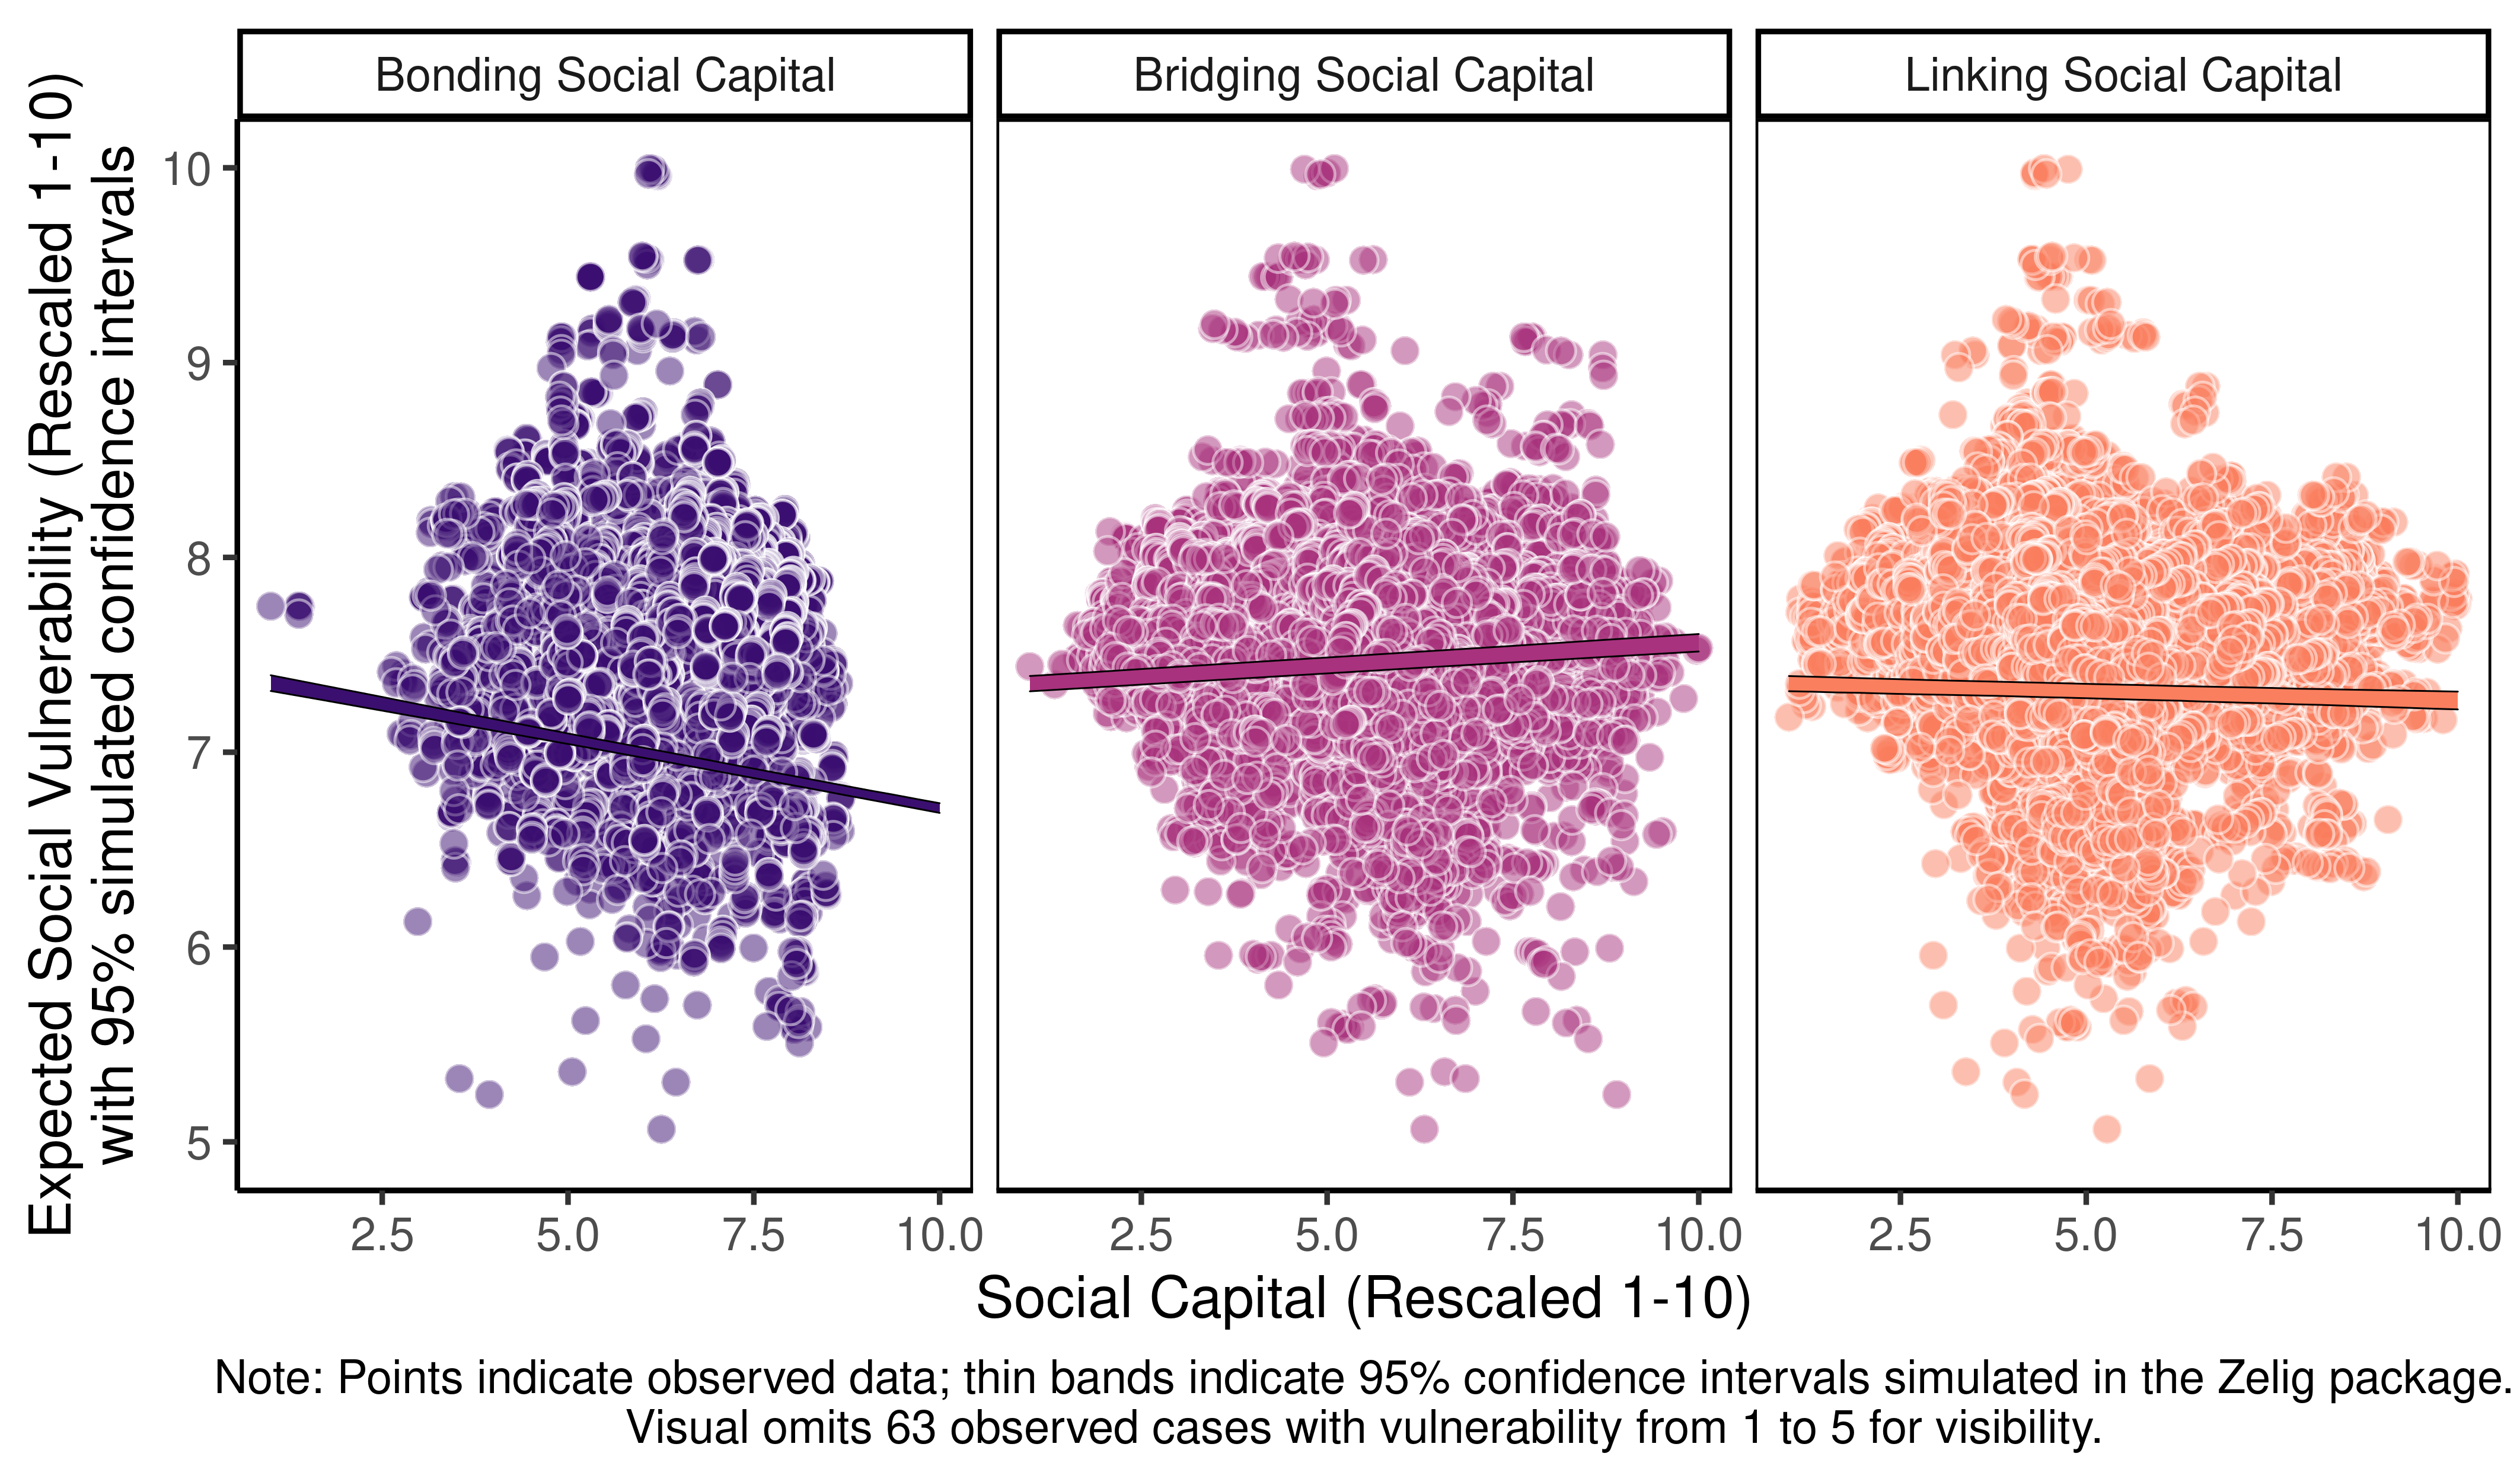
\includegraphics[width=1\linewidth]{fixed_effect_ev} \caption{Figure A1: Simulated Effects in Fixed Effects Models (Validation Model 8)}\label{fig:figa1}
\end{figure}
\elandscape


\end{document}
